\chapter{Search}
This chapter is the first of three chapters where we will solve problems by making use of
\blue{declarative programming}. \index{declarative programming}
The idea of declarative programming is that rather than developing a program to solve a specific problem,
we implement an algorithm that can solve a whole class of problems.  Then, in order to solve a problem that
falls within this class, we just have to specify the problem, which is usually much easier than solving it from
scratch.  In this chapter, this idea is illustrated via \blue{search problems}.
First, we define the notion of a \blue{search problem} formally.  This notion is then illustrated with two
examples.  We start with the \blue{missionaries and cannibals problem}.  Next, we use the 
\href{https://en.wikipedia.org/wiki/15_puzzle}{sliding puzzle} as our running example. \index{sliding puzzle}
After that we introduce various algorithms for solving search problems.  In particular, we present
\begin{enumerate}
\item \blue{breadth first search},
\item \blue{depth first search},
\item \blue{iterative deepening},
\item \blue{bidirectional breadth first search},
\item \blue{$\mathrm{A}^*$ search} and \blue{bidirectional $\mathrm{A}^*$ search},
\item \blue{iterative deepening $\mathrm{A}^*$ search}, and
\item \blue{$\mathrm{A}^*$-$\mathrm{IDA}^*$ search}.
\end{enumerate}

\begin{Definition}[Search Problem]
  A \blue{search problem} \index{search problem} is a tuple of the form
  \\[0.2cm]
  \hspace*{1.3cm}
  $\mathcal{P} = \langle Q,\;\mathtt{next\_states},\; \mathtt{start},\; \mathtt{goal}\rangle$
  \\[0.2cm]
  where
  \begin{enumerate}
  \item $Q$ is the set of \blue{states}, also known as the \blue{state space}.
        \index{state}
  \item \textts{next\_states} is a function taking a state as input and returning the set of those
        states that can be reached from the given state in one step,
        i.e.~we have
        \\[0.2cm]
        \hspace*{1.3cm}
        $\texttt{next\_states}:Q \rightarrow 2^Q$.
        \\[0.2cm]
        The function \textts{next\_states} gives rise to the \blue{transition relation} $R$, which is a
        relation on $Q$, i.e.~we have $R \subseteq Q \times Q$.  This relation is defined as follows:
        \\[0.2cm]
        \hspace*{1.3cm}
        $R := \bigl\{ \pair(s_1, s_2) \in Q \times Q \mid s_2 \in \mathtt{next\_states}(s_1) \bigr\}$.
        \\[0.2cm]
        If either $\pair(s_1, s_2) \in R$ or $\pair(s_2, s_1) \in R$, then  $s_1$ and $s_2$ are
        called \blue{neighboring states}.
        \index{\texttt{next\_states}}
  \item \textts{start} is the \blue{start state}, hence $\mathtt{start} \in Q$.
        \index{start state}
  \item \textts{goal} is the \blue{goal state}, hence $\mathtt{goal} \in Q$.
        \index{goal state}
    
        Sometimes, instead of a single $\mathtt{goal}$ there is a set of goal states $\mathtt{Goals}$.
  \end{enumerate}
  A \blue{path} \index{path} is a list $[s_1, \cdots, s_n]$ such that $s_{i+1} \in \mathtt{next\_states}(s_i)$ for all $i \in
  \{1,\cdots,n-1\}$.
  \index{path}
  The \blue{length} of this path is defined as the length of this list.
  A path $[s_1, \cdots, s_n]$ is a \blue{solution} \index{solution, of a search problem}
  to the search problem $P$ iff \index{search problem, solution}
  the following conditions are satisfied:
  \begin{enumerate}
  \item $s_1 = \mathtt{start}$, i.e.~the first element of the path is the start state.
  \item $s_n = \mathtt{goal}$, i.e.~the last element of the path is the goal state.

        If instead of a single $\mathtt{goal}$ we have a set of $\mathtt{Goals}$, then the last condition
        is changed into
        \\[0.2cm]
        \hspace*{1.3cm}
        $s_n \in \mathtt{Goals}$.
  \end{enumerate}
  A path $p = [s_1, \cdots, s_n]$ is a \blue{minimal solution} to the search problem $\mathcal{P}$
  \index{solution, minimal}
  iff it is a solution and, furthermore, the length of $p$ is minimal among all other solutions. \eoxs
\end{Definition}

\remark
In the literature, a \blue{state} is often called a \blue{node}.  \index{node}
In these lecture notes, I will also refer to states as nodes.  \eoxs

\example
We illustrate the notion of a search problem with the following example, which is also known as the
\href{https://en.wikipedia.org/wiki/Missionaries_and_cannibals_problem}{missionaries and cannibals problem}:
\index{missionaries and cannibals}
Three missionaries and three infidels have to cross a river that runs from the north to the south.
Initially, both the missionaries and the infidels are on the western shore.  There is just one small boat 
that can carry at most two passengers.  Both the missionaries and the infidels can steer the boat.
However, if at any time the missionaries are confronted with a majority of infidels on either shore of the
river, then the missionaries have a problem.

\begin{figure}[!ht]
\centering
\begin{Verbatim}[ frame         = lines,
                  framesep      = 0.3cm,
                  firstnumber   = 1,
                  labelposition = bottomline,
                  numbers       = left,
                  numbersep     = -0.2cm,
                  xleftmargin   = 0.8cm,
                  xrightmargin  = 0.8cm,
                ]
    problem = lambda m, i: 0 < m < i

    noProblem = lambda m, i: not problem(m, i) and not problem(3 - m, 3 - i)

    def next\_states(state):
        m, i, b = state
        if b == 1:
            return { (m - mb, i - ib, 0) for mb in range(m+1)
                                         for ib in range(i+1)
                                         if 1 <= mb + ib <= 2 and 
                                            noProblem(m - mb, i - ib) 
                   }
        else:
            return { (m + mb, i + ib, 1) for mb in range(3-m+1)
                                         for ib in range(3-i+1)
                                         if 1 <= mb + ib <= 2 and 
                                            noProblem(m + mb, i + ib) 
                   }

    start = (3, 3, 1)
    goal  = (0, 0, 0)
\end{Verbatim}
\vspace*{-0.3cm}
\caption{The missionary and cannibals problem coded as a search problem.}
\label{fig:missionaries.stlx}
\end{figure}
\noindent
Figure \ref{fig:missionaries.stlx} shows a formalization of the missionaries and cannibals problem
as a search problem.  We discuss this formalization line by line.
\begin{enumerate}
\item Line 1 defines the auxiliary function \textts{problem}.

      If $m$ is the number of missionaries on a given shore, while $i$ is the number of infidels on
      that same shore, then $\texttt{problem}(m, i)$ is \texttt{True} iff the missionaries have a problem on that
      shore.  There is a problem if the number of missionaries is greater than $0$ but less than the number of
      infidels. 
\item Line 3 defines the auxiliary function \textts{noProblem}.

      If $m$ is the number of missionaries on the western shore and $i$ is the number of infidels on
      that shore, then the expression $\texttt{noProblem}(m, i)$ is true, if there is no problem
      for the missionaries on either shore.

      The implementation of this function uses the fact that if $m$ is the number of missionaries on
      the western shore, then $3-m$ is the number of missionaries on the eastern shore.  Similarly,
      if $i$ is the number of infidels on the western shore, then the number of infidels on the
      eastern shore is $3 - i$.
\item Lines 5 to 18 define the function \textts{next\_states}.  A state $s$ is represented as a triple of
      the form
      \\[0.2cm]
      \hspace*{1.3cm}
      $s = (m, i, b)$ \quad where $m \in \{0,1,2,3\}$, $i \in \{0,1,2,3\}$, and $b \in\{0,1\}$.
      \\[0.2cm]
      Here $m$, $i$, and $b$ are, respectively, the number of missionaries, the number of infidels, and the number
      of boats on the western shore. 
      \begin{enumerate}[(a)]
      \item Line 6 extracts the components $m$, $i$, and $b$ from the state $s$.
      \item Line 7 checks whether the boat is on the western shore.
      \item If this is the case,  then the states reachable from the given state $s$ are those
            states where $\mathtt{mb}$ missionaries and $\mathtt{ib}$ infidels cross the river.
            After $\mathtt{mb}$ missionaries and $\mathtt{ib}$ infidels have crossed the river and
            reached the eastern shore, $\mathtt{m} - \mathtt{mb}$ missionaries and $\mathtt{i} - \mathtt{ib}$ infidels
            remain on the western shore.  Of course, after the crossing the boat is no longer on the
            western shore.  Therefore, the new state has the form
            \\[0.2cm]
            \hspace*{1.3cm}
            \texttt{(m - mb, i - ib, 0)}.
            \\[0.2cm]
            This explains line 8.
      \item Since the number $\mathtt{mb}$ of missionaries leaving the western shore can not be greater
            than the number $m$ of all missionaries on the western shore, we have the condition
            \\[0.2cm]
            \hspace*{1.3cm}
            $\mathtt{mb} \in \{0,\cdots,\mathrm{m}\}$,
            \\[0.2cm]
            which is implemented by the line
            \\[0.2cm]
            \hspace*{1.3cm}
            \texttt{for mb in range(m+1)}
            \\[0.2cm]
            There is a similar condition for the number of infidels crossing:
            \\[0.2cm]
            \hspace*{1.3cm}
            $\mathtt{ib} \in \{0,\cdots,\mathrm{i}\}$
            \\[0.2cm]
            which is implemented by
            \\[0.2cm]
            \hspace*{1.3cm}
            \texttt{for ib in range(i+1)}.
      \item Furthermore, we have to check that the number of persons crossing the river is at least 1
            and at most 2.  This explains the condition
            \\[0.2cm]
            \hspace*{1.3cm}
            \texttt{1 <= mb + ib <= 2}.
            \\[0.2cm]
            Finally, there should be no problem in the new state on either shore.  This is checked
            using the expression
            \\[0.2cm]
            \hspace*{1.3cm}
            \texttt{noProblem(m - mb, i - ib)}.
      \end{enumerate}
\item If the boat is on the eastern shore instead, then the missionaries and the infidels will be crossing
      the river from the eastern shore to the western shore.  Therefore, the number of missionaries and
      infidels on the western shore is now increased.  Hence, in this case the new state has the form
      \\[0.2cm]
      \hspace*{1.3cm}
      \texttt{(m + mb, i + ib, 1)}.
      \\[0.2cm]
      here, \texttt{mb} is the number of missionaries arriving on the western shore and \texttt{ib} is the
      number of arriving infidels.
      As the number of missionaries on the eastern shore is $3 - \mathrm{m}$ and the number of infidels on the
      eastern shore is $3 - \mathrm{i}$, $\mathtt{mb}$ has to be a member of the set $\{0,\cdots,3 -\mathtt{m}\}$, while
      $\mathtt{ib}$ has to be a member of the set $\{0,\cdots,3 - \mathtt{i}\}$.
\item Finally the start state and the goal state are defined in line 20 and line 21.
\end{enumerate}
The code in Figure \ref{fig:missionaries.stlx} does not define the set of states $Q$ of the search problem.  The
reason is that, in order to solve the problem, we do not need to define this set.  If we wanted to, we could
define the set of states as follows: 
\begin{verbatim}
    States = { (m, i, b) for m in {0, 1, 2, 3}
                         for i in {0, 1, 2, 3}
                         for b in {0, 1} 
                         if noProblem(m, i)
             }
\end{verbatim}
However, in general the set of states is not needed by the algorithms solving search problems and in many cases
this set is so big that it would be impossible to compute it.  Hence, in practice the set of states is only an
abstract notion that is needed in order to specify the function \texttt{next\_states}, but it is not implemented.

Figure \ref{fig:missionaries.pdf} shows a graphical representation of the transition relation of the
missionaries and cannibals puzzle.  In that figure, for every state both the western and the
eastern shore are shown.  The start state is covered with a blue ellipse, while the goal state is
covered with a green ellipse.  The figure clearly shows that the problem is solvable and that there
is a solution involving just 11 crossings of the river.
\eox

\begin{figure}[!ht]
  \centering
  \framebox{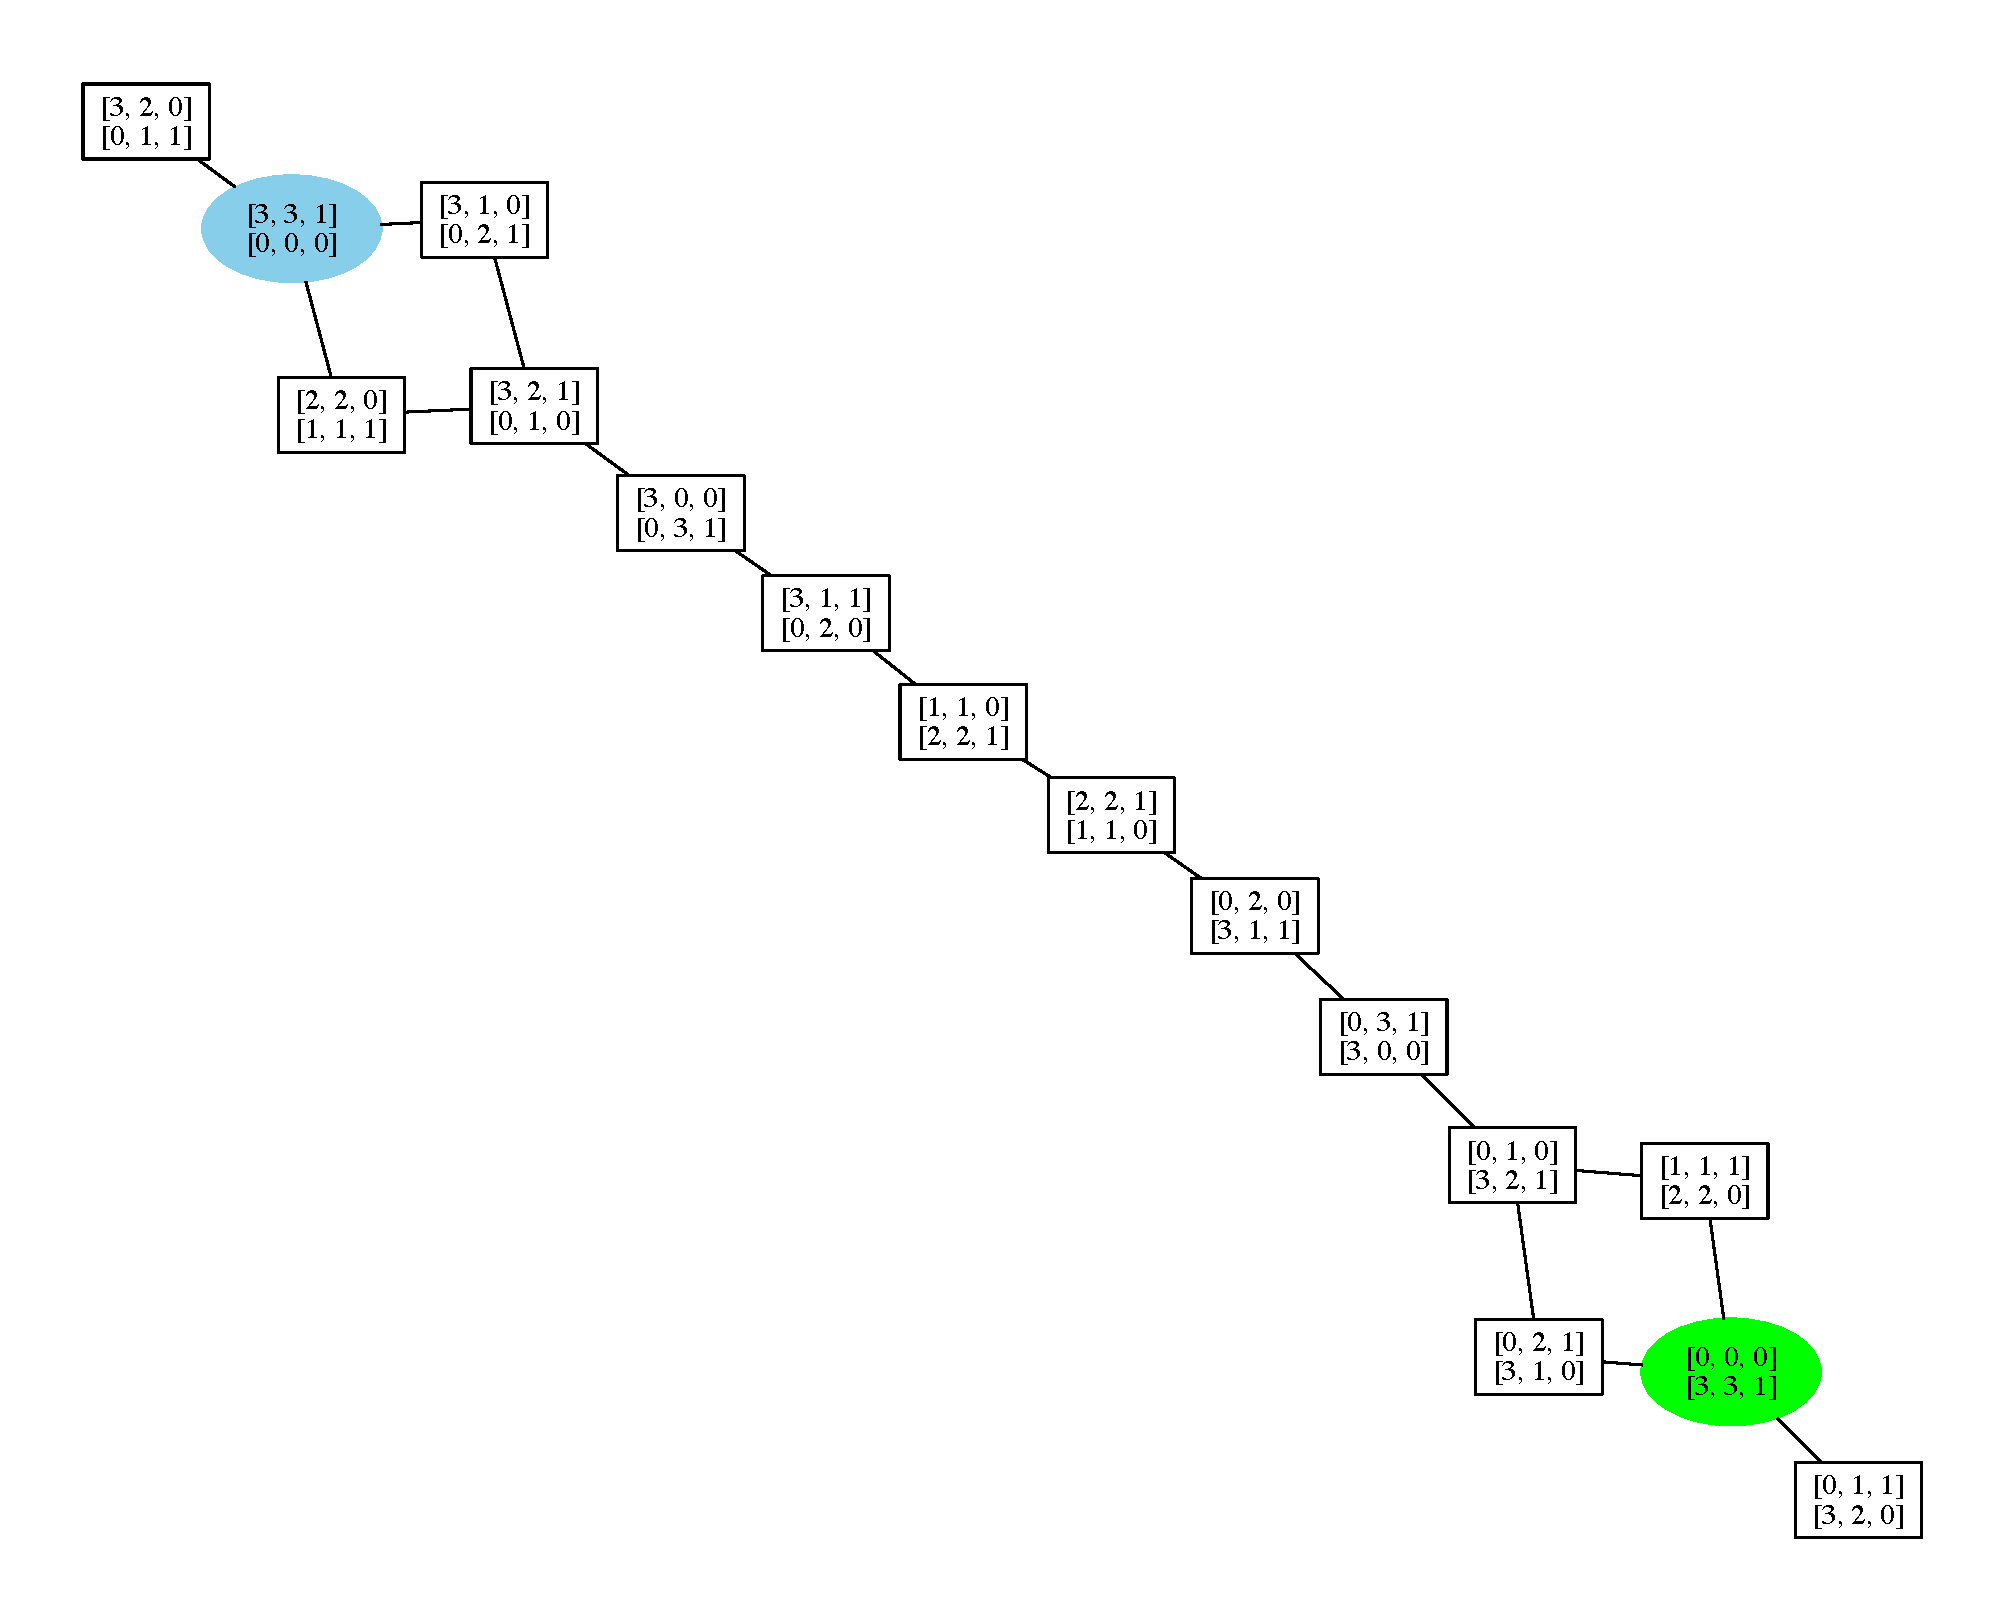
\epsfig{file=Figures/missionare.pdf,scale=0.5}}
  \caption{A graphical representation of the missionaries and cannibals problem.}
  \label{fig:missionaries.pdf}
\end{figure}


\section{The Sliding Puzzle}
The missionaries and cannibals problem is rather small and therefore it is not useful when we want to compare
the efficiency of various algorithms for solving search problems.  Therefore, we will now present a problem
that has a bigger complexity:  The $3 \times 3$ sliding puzzle uses a \index{sliding puzzle}
square board, where each side has a length of 3.  This board is subdivided into $3 \times 3 = 9$ squares of length 1.  Of
these 9 squares, 8 are occupied with square tiles that are numbered from 1 to 8.  One square remains
empty. Figure \ref{fig:8-puzzle.pdf} on page \pageref{fig:8-puzzle.pdf} shows two possible states of this
sliding puzzle.  The $4 \times 4$ \href{https://en.wikipedia.org/wiki/15_puzzle}{sliding puzzle}
is similar to the $3 \times 3$ sliding puzzle but uses a square board of size 4
instead.  The $4 \times 4$ sliding puzzle is also known as the \blue{15 puzzle}, while the $3 \times 3$ puzzle is
called the \blue{8 puzzle}. \index{8 puzzle} \index{15 puzzle}

\begin{figure}[!ht]
\centering
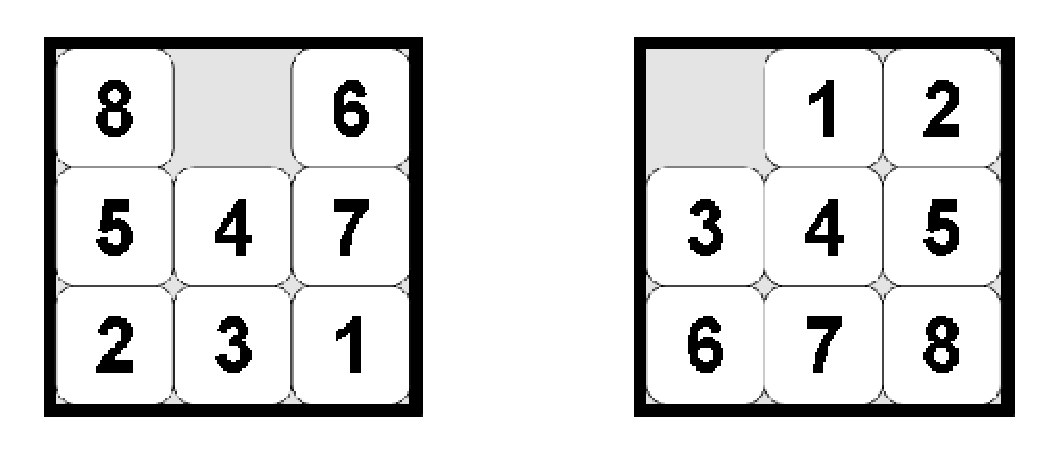
\epsfig{file=Figures/8-puzzle.pdf, scale=0.6}
\caption{The $3 \times 3$ sliding puzzle.}
\label{fig:8-puzzle.pdf}
\end{figure}

In order to \href{http://www.artbylogic.com/puzzles/numSlider/numberShuffle.htm?rows=3&cols=3&sqr=1}{solve} the $3 \times 3$ sliding puzzle shown in Figure \ref{fig:8-puzzle.pdf} we have to
transform the state shown on the left of Figure \ref{fig:8-puzzle.pdf} into the state shown on the
right of this figure.  The following operations are permitted when transforming a state of the
sliding puzzle:
\begin{enumerate}
\item If a tile is to the left  of the free square, this tile can be moved to the right.
\item If a tile is to the right of the free square, this tile can be moved to the left.
\item If a tile is above           the free square, this tile can be moved down.
\item If a tile is below           the free square, this tile can be moved up.
\end{enumerate}
In order to get a feeling for the complexity of the sliding puzzle, you can check the page
\\[0.2cm]
\hspace*{1.3cm}
\href{http://mypuzzle.org/sliding}{http://mypuzzle.org/sliding}.
\\[0.2cm]
The sliding puzzle is much more complex than the missionaries and cannibals problem because the
state space is much larger.  For the case of the $3 \times 3$ sliding puzzle, there are 9 squares
that can be positioned in $9!$ different ways.  It turns out that only half of these positions are
reachable from a given start state.  Therefore, the effective number of states for the $3 \times 3$
sliding puzzle is
\\[0.2cm]
\hspace*{1.3cm}
$9! / 2 = 181,440$.
\\[0.2cm]
This is already a big number, but $181,440$ states can still be stored on a modern computer.  However, the
$4 \times 4$ sliding puzzle has
\\[0.2cm]
\hspace*{1.3cm}
$16!/2 = 10,461,394,944,000$
\\[0.2cm]
different states reachable from a given start state.  If a state is represented as matrix containing
16 numbers and we store every number using just 4 bits, we still need $16 \cdot 4 = 64$ bits or 8
bytes for every state.  Hence we would need a total of
\\[0.2cm]
\hspace*{1.3cm}
$(16! / 2) \cdot 8 = 83,691,159,552,000$
\\[0.2cm]
bytes to store every state. We would thus need about 84 Terabytes to store the set of all states.  As few
computers are equipped with this kind of memory, it is obvious that we won't be able to store the
entire state space in memory.

\begin{figure}[!ht]
\centering
\begin{Verbatim}[ frame         = lines,
                  framesep      = 0.3cm,
                  firstnumber   = 1,
                  labelposition = bottomline,
                  numbers       = left,
                  numbersep     = -0.2cm,
                  xleftmargin   = 0.8cm,
                  xrightmargin  = 0.8cm,
                ]
    to_list = lambda State: [list(row) for row in State]
    
    to_tuple = lambda State: tuple(tuple(row) for row in State)
    
    def find_tile(tile, State):
        n = len(State)
        for row in range(n):
            for col in range(n):
                if State[row][col] == tile:
                    return row, col
    
    def move_dir(State, row, col, dx, dy):
        State = to_list(State)
        State[row     ][col     ] = State[row + dx][col + dy]
        State[row + dx][col + dy] = 0
        return to_tuple(State)
    
    def next_states(State):
        n          = len(State)
        row, col   = find_tile(0, State)
        New_States = set()
        Directions = [ (1, 0), (-1, 0), (0, 1), (0, -1) ]
        for dx, dy in Directions:
            if row + dx in range(n) and col + dy in range(n):
                New_States.add(move_dir(State, row, col, dx, dy))
        return New_States
    
    start = ( (8, 0, 6),
              (5, 4, 7),
              (2, 3, 1)
            )

    goal = ( (0, 1, 2), 
             (3, 4, 5), 
             (6, 7, 8)
           )
\end{Verbatim}
\vspace*{-0.3cm}
\caption{The $3 \times 3$ sliding puzzle.}
\label{fig:Sliding-Puzzle.ipynb}
\end{figure}
Figure \ref{fig:Sliding-Puzzle.ipynb} shows how the $3 \times 3$ sliding puzzle can be formulated as
a search problem.  In order to discuss the program, we first have to understand that states are
represented as tuples of tuples.  For example, the state shown above on the left side in Figure
\ref{fig:8-puzzle.pdf} is represented as the tuple:
\begin{verbatim}
        ( (8, 0, 6),
          (5, 4, 7),
          (2, 3, 1)
        )
\end{verbatim}
Here, we have represented the empty tile as $0$.
If states are represented as tuples of tuples, given a state $s$, the expression $s[r][c]$ returns the tile in
the row $r$ and column $c$, where counting of rows and columns starts from $0$.
We have to represent states as tuples of tuples rather than lists of lists since
tuples are immutable while lists are mutable and we need to store states in sets later.  In \textsl{Python},
sets can only store immutable objects.  However, later we have to manipulate the states.  To this end, we have
to first transform them to lists of lists, which can be manipulated.  After the manipulation these lists of
lists have to be transformed back to tuples of tuples.
We proceed to discuss the program shown in Figure \ref{fig:Sliding-Puzzle.ipynb} line by line.
\begin{enumerate}
\item The function \textts{to\_list} transforms a tuple of tuples into a list of lists.
\item The function \textts{to\_tuple} transforms a list of lists into a tuple of tuples.
\item \textts{findTile} is an auxiliary function that is needed to implement the function \textts{next\_states}.
      It is called with a $\mathtt{number}$ and a $\mathtt{State}$ and
      returns the row and column where the tile labelled with $\mathtt{number}$ can be found.
\item \textts{moveDir} takes a $\mathtt{State}$, the $\mathtt{row}$ and the $\mathtt{col}$umn
      where to find the empty square and a direction in which the empty square should be moved.
      This direction is specified via the two variables $\mathtt{dx}$ and $\mathtt{dy}$.  The tile
      at the position $\langle\mathtt{row} + \mathtt{dx}, \mathtt{col} + \mathtt{dy}\rangle$ is
      moved into the position $\langle\mathtt{row}, \mathtt{col}\rangle$, while the tile at position
      $\langle\mathtt{row} + \mathtt{dx}, \mathtt{col} + \mathtt{dy}\rangle$ becomes empty.
\item Given a $\mathtt{State}$, the function \textts{next\_states} computes the set of all states
      that can be reached in one step from $\mathtt{State}$.  The basic idea is to find the position of the
      empty tile and then try to move the empty tile in all possible directions.  If the empty tile is found at
      position $(\mathtt{row}, \mathtt{col})$ and the direction of the movement is given as $(\mathtt{dx}, \mathtt{dy})$, then
      in order to ensure that the empty tile can be moved to the position $[\mathtt{row}+\mathtt{dx}, \mathtt{col}+\mathtt{dy}]$,
      we have to ensure that both
      \\[0.2cm]
      \hspace*{1.3cm}
      $\mathtt{row}+\mathtt{dx} \in \{0,\cdots,n-1\}$ \quad and \quad
      $\mathtt{col}+\mathtt{dy} \in \{0,\cdots,n-1\}$
      \\[0.2cm]
      hold, where $n$ is the size of the board.
\end{enumerate}

Next, we want to develop an algorithm that can solve puzzles of the kind described so far.  The most basic
algorithm to solve search problems is \href{https://en.wikipedia.org/wiki/Breadth-first_search}{breadth first search}.
We discuss this algorithm next.

\section{Breadth First Search}
Informally, breadth first search, abbreviated as \ac{bfs}, works as follows: \index{breadth first search}
\begin{enumerate}
\item Given a search problems $\langle Q,\;\mathtt{next\_states},\; \mathtt{start},\; \mathtt{goal}\rangle$,
      we initialize a set $\mathtt{Frontier}$ to contain the state $\mathtt{start}$.

      In general, $\mathtt{Frontier}$ contains those states that have just been discovered and whose successors have not
      yet been seen.
\item As long as the set $\mathtt{Frontier}$ does not contain the state $\mathtt{goal}$, we recompute this set
      by adding all states to it that can be reached in one step from a state in $\mathtt{Frontier}$.
      Then, the states that had been previously present in $\mathtt{Frontier}$ are removed.
      These old states are then saved into a set $\mathtt{Visited}$.
\end{enumerate}
In order to avoid loops, an implementation of breadth first search keeps track of those states that have
been visited in the set $\mathtt{Visited}$.  Once a state has been added to
the set $\mathtt{Visited}$,  it will never be revisited again.
Furthermore, in order to keep track of the path leading to the goal, we utilize a dictionary called
$\mathtt{Parent}$.  For every state $s$ that is in $\mathtt{Frontier}$, $\mathtt{Parent}[s]$ is the state that
caused $s$ to be added to the set $\mathtt{Frontier}$, i.e.~for all states $s\in\mathtt{Visited}\cup\mathtt{Frontier}$ 
we have 
\\[0.2cm]
\hspace*{1.3cm}
$s \in \mathtt{next\_states}(\mathtt{Parent}[s])$.


\begin{figure}[!ht]
\centering
\begin{Verbatim}[ frame         = lines,
                  framesep      = 0.3cm,
                  firstnumber   = 1,
                  labelposition = bottomline,
                  numbers       = left,
                  numbersep     = -0.2cm,
                  xleftmargin   = 0.8cm,
                  xrightmargin  = 0.8cm,
                ]
    def search(start, goal, next_states):
        Frontier = { start }
        Visited  = set()
        Parent   = { start: start }
        while len(Frontier) > 0:
            NewFrontier = set()
            for s in Frontier:
                for ns in next_states(s):
                    if ns not in Visited and ns not in Frontier:
                        NewFrontier.add(ns)
                        Parent[ns] = s
                        if ns == goal:
                            return path_to(goal, Parent)
            Visited |= Frontier
            Frontier = NewFrontier
\end{Verbatim}
\vspace*{-0.3cm}
\caption{Breadth first search.}
\label{fig:Breadth-First-Search.ipynb}
\end{figure}
\myFig{Breadth-First-Search.ipynb} shows an implementation of
breadth first search in \textsl{Python}.  We discuss this implementation line by line:
\begin{enumerate}
\item $\mathtt{Frontier}$ is the set of all those states that have been encountered but whose
      neighbours have not yet been explored.  Initially, it contains the state $\mathtt{start}$.
\item $\mathtt{Visited}$ is the set of all those states, all whose neighbours have already been
      added to the set $\mathtt{Frontier}$.  In order to avoid infinite loops, these states must not
      be visited again.
\item $\mathtt{Parent}$ is a dictionary keeping track of the predecessors of the state that have been reached.
      The only state with no real predecessor is the state \texttt{start}.  By convention, \texttt{start} is its
      own predecessor.
\item As long as the set $\mathtt{Frontier}$ is not empty, we add all neighbours of states in
      $\mathtt{Frontier}$ that have not yet been visited to the set $\mathtt{NewFrontier}$.
      When doing this, we keep track of the path leading to a new state $\mathtt{ns}$ by storing its
      parent in the dictionary $\mathtt{Parent}$.
\item If the new state happens to be the state $\mathtt{goal}$, we return a path leading from
      $\mathtt{start}$ to $\mathtt{goal}$.  The function $\mathtt{pathTo}()$ is shown in Figure
      \ref{fig:pathTo.stlx} on page \pageref{fig:pathTo.stlx}.
\item After we have collected all successors of states in $\mathtt{Frontier}$, the states
      in the set $\mathtt{Frontier}$ have been visited and are therefore added to the set
      $\mathtt{Visited}$, while the set $\mathtt{Frontier}$ is updated to $\mathtt{NewFrontier}$.
\end{enumerate}

\begin{figure}[!ht]
\centering
\begin{Verbatim}[ frame         = lines,
                  framesep      = 0.3cm,
                  firstnumber   = 1,
                  labelposition = bottomline,
                  numbers       = left,
                  numbersep     = -0.2cm,
                  xleftmargin   = 0.8cm,
                  xrightmargin  = 0.8cm,
                ]
    def path_to(state, Parent):
        p = Parent[state]
        if p == state:
            return [state]
        return path_to(p, Parent) + [state]
\end{Verbatim}
\vspace*{-0.3cm}
\caption{The function $\mathtt{pathTo}()$.}
\label{fig:pathTo.stlx}
\end{figure}
The function call $\mathtt{pathTo}(\mathtt{state}, \mathtt{Parent})$ constructs a path reaching
from $\mathtt{start}$ to $\mathtt{state}$ in reverse by looking up the parent states.

If we try breadth first search to solve the missionaries and cannibals problem, we obtain
the solution shown in Figure \ref{fig:missionaries.solution}.  15 nodes had to be expanded to find
this solution.  To keep this in perspective, we note that Figure \ref{fig:missionaries.pdf} shows
that the entire state space contains 16 states.  Therefore, with the exception of one state, we have
inspected all the states.  This is a typical behaviour for breadth first search.

\begin{figure}[!ht]
\centering
\begin{Verbatim}[ frame         = lines,
                  framesep      = 0.3cm,
                  firstnumber   = 1,
                  labelposition = bottomline,
                  numbers       = left,
                  numbersep     = -0.2cm,
                  xleftmargin   = 0.8cm,
                  xrightmargin  = 0.8cm,
                ]
    MMM   KKK   B      |~~~~~|
                       >  KK >
    MMM   K            |~~~~~|              KK  B
                       <  K  <
    MMM   KK    B      |~~~~~|               K
                       >  KK >
    MMM                |~~~~~|             KKK  B
                       <  K  <
    MMM   K     B      |~~~~~|              KK
                       > MM  >
    M     K            |~~~~~|        MM    KK  B
                       < M K <
    MM    KK    B      |~~~~~|         M     K
                       > MM  >
          KK           |~~~~~|       MMM     K  B
                       <  K  <
          KKK   B      |~~~~~|       MMM
                       >  KK >
          K            |~~~~~|       MMM    KK  B
                       <  K  <
          KK    B      |~~~~~|       MMM     K
                       >  KK >
                       |~~~~~|       MMM   KKK  B
\end{Verbatim}
\vspace*{-0.3cm}
\caption{A solution of the missionaries and cannibals problem.}
\label{fig:missionaries.solution}
\end{figure}

Next, let us try to solve the $3 \times 3$ sliding puzzle.  It takes about 2 seconds to solve
this problem on my computer\footnote{
  I happen to own an iMac from 2017.  This iMac is equipped with 32 Gigabytes of main memory and a
  quad core 3.4 GHz ``Intel Core i5'' processor.  I suspect this to be the I5-7500 (Kaby Lake) processor.
}, while 181,439 states are touched.  Again, we see that breadth first search touches nearly all the
states reachable from the start state.

Breadth first search has two important properties:
\begin{enumerate}
\item Breadth first search is \blue{complete}:  If there is a solution to the given
      search problem, then breadth first search is going to find it.
\item The solution found by breadth first search is \blue{optimal}, i.e.~it is one of the
      shortest possible solutions.
\end{enumerate}
\proof
Both of these claims can be shown simultaneously.  Consider the implementation of breadth first
search shown in Figure \ref{fig:Breadth-First-Search.ipynb}.  An easy induction on the number of
iterations of the \texttt{while} loop shows that after $n$ iterations of the \texttt{while} loop,
the set $\mathtt{Frontier}$ contains exactly those states that have a distance of $n$ to the state
$\mathtt{start}$.  This claim is obviously true before the first iteration of the while loop as in
this case, $\mathtt{Frontier}$ only contains the state $\mathtt{start}$.  In the induction step we
assume the claim is true after $n$ iterations.  Then, in the next iteration all states that can be
reached in one step from a state in $\mathtt{Frontier}$ are added to the new $\mathtt{Frontier}$,
provided there is no shorter path to them.  There is a shorter path to a state if this
state is already a member of the set $\mathtt{Visited}$.  Otherwise, the shortest path to a state that is
reached in iteration $n+1$ has the length $n+1$.  Hence, the claim is true after $n+1$
iterations also.

Now, if there is a path from $\mathtt{start}$ to $\mathtt{goal}$, there must also be a shortest
path.  Assume this path has a length of $k$.  Then, $\mathtt{goal}$ is reached in the iteration
number $k$ and the shortest path is returned.
\qed

The fact that breadth first search is both complete and the path returned is optimal is rather
satisfying.  However, breadth first search still has a big downside that makes it unusable for
many problems:  If the \texttt{goal} is far from the $\mathtt{start}$, breadth first search will use
a lot of memory because it will store a large part of the state space in the set
$\mathtt{Visited}$.  In many cases, the state space is so big that this is not possible.  For example, it is
impossible to solve the more interesting cases of the $4 \times 4$ sliding puzzle using breadth first search.

\subsection{A Queue Based Implementation of Breadth First Search}
In the literature, for example in Figure 3.11 of Russell \& Norvig \cite{russell:2009}, breadth
first search is often implemented using a
\href{https://en.wikipedia.org/wiki/Queue_(abstract_data_type)}{queue} data structure.
Figure \ref{fig:Breadth-First-Search-Queue.ipynb} on page
\pageref{fig:Breadth-First-Search-Queue.ipynb} shows an implementation of breadth first search that
uses a queue to store the set \texttt{Frontier}.   Here we use the module \texttt{deque} from the package
\texttt{collections}. This module implements a
\href{https://en.wikipedia.org/wiki/Double-ended_queue}{double-ended queue}, \index{double-ended queue}
which is implemented as a 
\href{https://en.wikipedia.org/wiki/Doubly_linked_list}{doubly linked list}. \index{doubly linked list}
Besides the constructor, our
implementation uses two methods from the class \texttt{deque}:
\begin{enumerate}
\item Line 4 initializes the \texttt{Frontier} as a double-ended queue that contains the state \texttt{start}.
\item In line 8 we remove the oldest element in the queue \texttt{Frontier}, which is supposed to be at the
      left end of the queue.  This is achieved via the method \textts{popleft}.
\item In line 16 we add the states that have not been encountered previously at the right end of the queue
      \texttt{Frontier} using the method \textts{append}.
\end{enumerate}

\begin{figure}[!ht]
\centering
\begin{Verbatim}[ frame         = lines,
                  framesep      = 0.3cm,
                  firstnumber   = 1,
                  labelposition = bottomline,
                  numbers       = left,
                  numbersep     = -0.2cm,
                  xleftmargin   = 0.8cm,
                  xrightmargin  = 0.8cm,
                  ]
    from collections import deque
                  
    def search(start, goal, next_states):
        Frontier = deque([start])
        Visited  = set()
        Parent   = { start: start }
        while len(Frontier) > 0:
            state = Frontier.popleft()
            if state == goal:
                return path_to(state, Parent)
            Visited.add(state)
            newStates = next_states(state)
            for ns in newStates:
                if ns not in Visited and ns not in Parent:
                    Parent[ns] = state
                    Frontier.append(ns)
\end{Verbatim}
\vspace*{-0.3cm}
\caption{A queue based implementation of breadth first search.}
\label{fig:Breadth-First-Search-Queue.ipynb}
\end{figure}



\section{Depth First Search}
To overcome the memory limitations of breadth first search, the
\href{https://en.wikipedia.org/wiki/Depth-first_search}{depth first search} algorithm \index{depth first search}
has been developed.  Depth first search is abbreviated as \ac{dfs}.  There are two ideas involved when going from
breadth first search to depth first search:
\begin{enumerate}
\item In order to save memory, \ac{dfs} removes the set \texttt{Visited} of \ac{bfs}.
\item While \ac{bfs} ensures that every state is visited by implementing the \texttt{Frontier} as a queue,
      \ac{dfs} replaces this queue by a stack.  This way, \ac{dfs} tries to get as far away from the state
      \texttt{start} as early as possible.  In order to prevent loops, we still have the parent dictionary.
\end{enumerate}
The resulting algorithm is shown in Figure
\ref{fig:Depth-First-Search-Stack.ipynb} on page \pageref{fig:Depth-First-Search-Stack.ipynb}.  Basically, in this
implementation, a path is searched to its end before trying an alternative.  This way, we might be able to find a
$\mathtt{goal}$ that is far away from $\mathtt{start}$ without exploring the whole state space.

\begin{figure}[!ht]
\centering
\begin{Verbatim}[ frame         = lines,
                  framesep      = 0.3cm,
                  firstnumber   = 1,
                  labelposition = bottomline,
                  numbers       = left,
                  numbersep     = -0.2cm,
                  xleftmargin   = 0.8cm,
                  xrightmargin  = 0.8cm,
                ]
    def search(start, goal, next_states):
        Stack  = deque([start])
        Parent = { start: start }
        while len(Stack) > 0:
            state = Stack.pop()
            for ns in next_states(state):
                if ns == goal:
                    return path_to(state, Parent) + [goal]
                if ns not in Parent:
                    Parent[ns] = state
                    Stack.append(ns)
\end{Verbatim}
\vspace*{-0.3cm}
\caption{The depth first search algorithm.}
\label{fig:Depth-First-Search-Stack.ipynb}
\end{figure}
The implementation of  \texttt{search} works as follows:
\begin{enumerate}
\item Any states that are encountered during the search are placed on top of the stack \texttt{Stack}.
\item In order to record the information how a state has been added to the \texttt{Stack}, we have a dictionary
      \texttt{Parent}.  For every state $s$ that is on \texttt{Stack}, $\texttt{Parent}[s]$ returns a state $p$
      such that $s \in \texttt{next\_states}(p)$,  i.e. $p$ is the state that immediately precedes $s$ on the
      path that leads from \texttt{start} to $s$.  
\item Initially, \texttt{Stack} only contains the state \texttt{start}.
\item As long as \texttt{Stack} is not empty, the \texttt{state} on top of \texttt{Stack} is replaced by all
      states that be reached in one step from \texttt{state}.  However, in order to prevent depth first search
      to run in circles, only those states \texttt{ns}from the set \texttt{next\_states(state)} are appended to
      \texttt{Stack} that have not been encountered previously.  This is checked by testing 
      whether \texttt{ns} is in the domain of \texttt{Parent}.
\item When the \texttt{goal} is reached,  a path leading from \texttt{start} to \texttt{goal} is returned.
\end{enumerate}
When we test the implementation shown above with the $3 \times 3$ sliding puzzle, it takes about 0.25 seconds
on my computer to find a solution.  This is quite an improvement compared to breadth first search.
Furthermore, there is no longer a need to keep the set $\mathtt{Visited}$ around, hence the memory requirements of depth
first search are much smaller than the memory requirements of breadth first search.  However, we still have
to maintain the set $\mathtt{Parent}$.  Fortunately, we will be able to get rid of the set $\mathtt{Parent}$ when we develop a recursive
implementation of depth first search in the following subsection.

However, there is also bad news: the solution that is found has a length of more than $8,000$ steps.  As the
shortest path from $\mathtt{start}$ to $\mathtt{goal}$ has only 31 steps, the solution found by depth
first search is very far from being optimal.

\subsection{A Recursive Implementation of Depth First Search}
Sometimes, the depth first search algorithm is presented as a recursive algorithm, since this leads
to an implementation that is slightly shorter and is easier to understand.  What is more, we no
longer need the dictionary $\mathtt{Parent}$ to record the parent of each node.  The resulting
implementation is shown in \myFig{depth-first-search-recursive.stlx}.

\begin{figure}[!ht]
\centering
\begin{Verbatim}[ frame         = lines,
                  framesep      = 0.3cm,
                  firstnumber   = 1,
                  labelposition = bottomline,
                  numbers       = left,
                  numbersep     = -0.2cm,
                  xleftmargin   = 0.8cm,
                  xrightmargin  = 0.8cm,
                ]
    def search(start, goal, next_states):
        return dfs(start, goal, next_states, [start])
    
    def dfs(state, goal, next_states, Path):
        if state == goal:
            return Path
        for ns in next_states(state):
            if ns not in Path:
                Result = dfs(ns, goal, next_states, Path + [ns])
                if Result != None:
                    return Result
\end{Verbatim}
\vspace*{-0.3cm}
\caption{A recursive implementation of depth first search.}
\label{fig:depth-first-search-recursive.stlx}
\end{figure}
The only purpose of the function \texttt{search} is to call the function $\mathtt{dfs}$, which needs one
additional argument.  This argument is called $\mathtt{Path}$.  The idea is that $\mathtt{Path}$ is
a path leading from the state $\mathtt{start}$ to the current $\mathtt{state}$ that is the first
argument of the function $\mathtt{dfs}$.  On the first invocation of $\mathtt{dfs}$, the
parameter $\mathtt{state}$ is equal to $\mathtt{start}$ and therefore $\mathtt{Path}$ is initialized
as the list containing only $\mathtt{start}$.

The implementation of $\mathtt{dfs}$ works as follows:
\begin{enumerate}
\item If $\mathtt{state}$ is equal to $\mathtt{goal}$, our search is successful. Since by assumption
      the list $\mathtt{Path}$ is a path connecting $\mathtt{start}$ and $\mathtt{state}$ and we
      have checked that $\mathtt{state}$ is equal to $\mathtt{goal}$, we can return $\mathtt{Path}$ as our solution.
\item Otherwise, $\mathtt{next\_states}(\mathtt{state})$ is the set of states that are reachable from $\mathtt{state}$
      in one step.  Any of the states $\mathtt{ns}$ in this set could be the next state on a path
      that leads to $\mathtt{goal}$.  Therefore, we try recursively to reach $\mathtt{goal}$ from
      every state $\mathtt{ns}$.  Note that we have to change $\mathtt{Path}$ to the list
      \\[0.2cm]
      \hspace*{1.3cm}
      \texttt{Path + [ns]}
      \\[0.2cm]
      when we call the function $\mathtt{dfs}$ recursively.  This way, we retain the invariant of
      $\mathtt{dfs}$ that the list $\mathtt{Path}$ is a path connecting $\mathtt{start}$ with $\mathtt{state}$.
\item We still have to avoid running in circles.  In the recursive version of depth first search,
      this is achieved by checking that the state $\mathtt{ns}$ is not already a member of the list $\mathtt{Path}$.  In the
      non-recursive version of depth first search, we had used the set $\mathtt{Parent}$ instead.
      The current implementation no longer has a need for the dictionary $\mathtt{Parent}$.  This is very
      fortunate since it reduces the memory requirements of depth first search considerably.
\item If one of the recursive calls of $\mathtt{dfs}$ returns a list, this list is a solution to our
      search problem and hence it is returned.  However, if instead 
      $\mathtt{None}$ is returned, the \texttt{for} loop needs to carry on and test the other
      successors of $\mathtt{state}$.
\item Note that the recursive invocation of $\mathtt{dfs}$ returns $\mathtt{None}$ if the end of the
      \texttt{for} loop is reached and no solution has been returned so far.  The reason is that there is
      no \texttt{return} statement at the end of the function $\mathtt{dfs}$.  Hence, if the last
      line of the function $\mathtt{dfs}$ is reached, $\mathtt{None}$ is returned by default.
\end{enumerate}

For the $3 \times 3$ puzzle, the recursive implementation takes about 26 second to compute the solution.  In
this case, the solution has a length of more than $20\,000$ steps.  This, together with the fact that function
calls are quite expensive in \textsl{Python}, is the reason that the recursive version is less efficient than
the stack based implementation of depth first search.
The good news is that this program does not need much memory.  The only variable that uses considerable memory
is the variable $\mathtt{Path}$.  If we can somehow keep the list $\mathtt{Path}$ short, then the recursive
version of depth first search uses only a small fraction of the memory needed by breadth first search.

\section{Iterative Deepening}
The fact that the recursive version of depth first search took just one second to find a solution is very
impressive.  The questions is whether it might be possible to force depth first search to find the shortest
solution.  The answer to this question leads to an algorithm that is known as
\href{https://en.wikipedia.org/wiki/Iterative_deepening_depth-first_search}{iterative deepening}.
\index{iterative deepening} The main idea behind iterative deepening is to run depth first with a \blue{depth
  limit} $d$.  This limit enforces that a solution has at most a length of $d$.  If no solution is found at a
depth of $d$, the new depth $d+1$ can be tried next and the process can be continued until a solution is found.
The program shown in Figure \ref{fig:Iterative-Deepening.ipynb} on page \pageref{fig:Iterative-Deepening.ipynb}
implements this strategy.  We proceed to discuss the details of this program.

\begin{figure}[!ht]
\centering
\begin{Verbatim}[ frame         = lines,
                  framesep      = 0.3cm,
                  firstnumber   = 1,
                  labelposition = bottomline,
                  numbers       = left,
                  numbersep     = -0.2cm,
                  xleftmargin   = 0.8cm,
                  xrightmargin  = 0.8cm,
                ]
    def search(start, goal, next_states):
        limit = 1
        while True:
            Path = depth_limited_search(start, goal, next_states, limit)
            if Path != None:
                return Path
            limit += 1
    
    def depth_limited_search(state, goal, next_states, limit):
        Stack = deque([[start]])
        while len(Stack) > 0:
            Path  = Stack.pop()
            state = Path[-1]
            if state == goal:
                return Path
            if len(Path) >= limit:
                continue
            for ns in next_states(state):
                if ns not in Path:
                    Stack.append(Path + [ns])
\end{Verbatim}
\vspace*{-0.3cm}
\caption{Iterative deepening implemented in \textsl{Python}.}
\label{fig:Iterative-Deepening.ipynb}
\end{figure}

\begin{enumerate}
\item The function $\mathtt{search}$ initializes the variable $\mathtt{limit}$ to 1 and tries to find a solution
      to the search problem that has a length that is less than or equal to $\mathtt{limit}$.  If a solution is
      found, it is returned.  Otherwise, the variable $\mathtt{limit}$ is incremented by one and a
      new instance of depth first search is started.  This process continues until either
      \begin{itemize}
      \item a solution is found \qquad or
      \item the sun rises in the west.
      \end{itemize}
\item The function $\mathtt{depthLimitedSearch}$ implements depth first search but takes care to compute only
      those paths that have a length of at most $\mathtt{limit}$.  The implementation shown in Figure
      \ref{fig:Iterative-Deepening.ipynb} is stack based.  In this implementation,
      the stack contains paths leading from $\mathtt{start}$ to the state at the end of a given
      path.  Hence it is similar to the implementation of depth first search shown in
      \myFig{Depth-First-Search-Stack.ipynb}.
\item The stack is initialized to contain the path $\mathtt{[start]}$.
\item In the \texttt{while}-loop, the first thing that happens is that the $\mathtt{Path}$ on top of
      the stack is removed from the stack.  The state at the end of this $\mathtt{Path}$ is called $\mathtt{state}$.
      If this $\mathtt{state}$ happens to be the $\mathtt{goal}$, a solution to the search problem
      has been found and this solution is returned.
\item Otherwise, we check the length of $\mathtt{Path}$.  If this length is greater than or equal to the
      $\mathtt{limit}$, the $\mathtt{Path}$ can be discarded as we have already checked that it
      does not end in the $\mathtt{goal}$.
\item Next, the neighbours of $\mathtt{state}$ are computed.  For every neighbour $\mathtt{ns}$
      of $\mathtt{state}$ that has not yet been encountered in $\mathtt{Path}$, we extend
      $\mathtt{Path}$ to a new list that ends in $\mathtt{ns}$ and push this new list onto the $\mathtt{Stack}$.
\item This process is iterated until the $\mathtt{Stack}$ is exhausted.
\end{enumerate}
The nice thing about the program presented in this section is the fact that it does not use much
memory.  The reason is that the stack can never have a size that is longer than $\mathtt{limit}$ and
therefore the overall memory that is needed can be bounded by $\mathcal{O}(\mathtt{limit}^2)$.
However, when we run this program to solve the $3 \times 3$ sliding puzzle, the algorithm takes
about 17 minutes.  There are two reasons for this:
\begin{enumerate}
\item First, it is quite wasteful to run the search for a depth limit of $1$, $2$, $3$, $\cdots$ all the way up
      to 31.  Essentially, all the computations done with a limit less than $31$ are wasted. However,
      this process is not as wasteful as we might first expect.  To see this, assume that the number of states
      reached is doubled\footnote{
        When we run breadth first search for the sliding puzzle we can observe that at least at the beginning
        of the search the number of states is roughly doubled after each step.  This observation holds true for
        the first 16 steps. 
      }
      after every iteration.  Then the number of states to explore when searching with a depth limit of $d$ is 
      roughly $2^d$.  Hence, when we run depth limited search up to depth $d$, the number of states visited is 
      \\[0.2cm]
      \hspace*{1.3cm}
      $\ds 1 + 2^1 + 2^2 + \cdots + 2^d = \sum\limits_{i=0}^d 2^i = 2^{d+1} - 1$.
      \\[0.2cm]
      Therefore, if the solution is found at a depth of $d+1$, we will explore roughly $2^{d+1}$ states to find
      the solution if we would do depth first search with a depth limit of $d+1$.  If, instead, we use
      iterative deepening, we have wastefully explored an additional number of $2^{d+1} -1$ states.  Hence, we
      will visit only twice the number of states with iterative deepening than we would have visited with depth
      limited search with the correct depth limit.
\item Given a state $s$ that is reachable from the $\mathtt{start}$, there often are a huge number of
      different paths that lead from $\texttt{start}$ to $s$.  The version of iterative deepening presented in
      this section tries all of these paths and hence needs a large amount of time.
\end{enumerate}

\exercise
Assume the set of states $Q$ is defined as
\\[0.2cm]
\hspace*{1.3cm}
$Q := \bigl\{ \pair(a, b) \mid a \in \mathbb{N} \wedge b \in \mathbb{N} \bigr\}$.
\\[0.2cm]
Furthermore, the states $\mathtt{start}$ and $\mathtt{goal}$ are defined as
\\[0.2cm]
\hspace*{1.3cm}
$\mathtt{start} := \pair(0,0)$ \quad and \quad $\mathtt{goal} := \pair(n,n)$ where $n \in \mathbb{N}$.
\\[0.2cm]
Next, the function $\mathtt{next\_states}$ is defined as
\\[0.2cm]
\hspace*{1.3cm}
$\mathtt{next\_states}\bigl(\pair(a,b)\bigr) := \bigl\{\pair(a+1,b), \pair(a,b+1)\bigr\}$.
\\[0.2cm]
Finally, the search problem $\mathcal{P}$ is defined as
\\[0.2cm]
\hspace*{1.3cm}
$\mathcal{P} := \langle Q, \mathtt{next\_states}, \mathtt{start}, \mathtt{goal} \rangle$.
\\[0.2cm]
Given a natural number $n$, compute the number of different solutions of this search problem and prove
your claim.  

\hint
The expression giving the number of different solutions contains factorials.  In order to get a better feeling
for the asymptotic growth of this expression we can use 
\href{https://en.wikipedia.org/wiki/Stirling%27s_approximation}{Stirling's approximation} of the factorial.
Stirling's approximation of $n!$ is given as follows: \index{Stirling's approximation of the factorial}
\\[0.2cm]
\hspace*{1.3cm}
$\ds n! \sim \sqrt{2 \cdot \pi \cdot n\,} \cdot \Bigl(\frac{n}{e}\Bigr)^n$.
\eox

\exercise
If there is no solution, the implementation of iterative deepening that is shown in Figure
\ref{fig:Iterative-Deepening.ipynb} does not terminate.  The reason is that the function $\mathtt{depthLimitedSearch}$ does not
distinguish between the following two reasons for failure:
\begin{enumerate}
\item It can fail to find a solution because the depth limit is reached.
\item It can also fail because it has tried all paths without hitting the depth limit but the $\mathtt{Stack}$ is exhausted.
\end{enumerate}
Improve the implementation of iterative deepening so that it will always terminate eventually, provided the
state space is finite.
\eoxs


\section{Bidirectional Breadth First Search}
Breadth first search first visits all states that have a distance of 1 from start, then all
states that have a distance of 2, then of 3 and so on until finally the goal is found.  If the length of the shortest path
from $\mathtt{start}$ to $\mathtt{goal}$ is $d$, then all states that have a distance of at most $d$ will be
visited.  In many search problems, the number of states grows exponentially with the distance, i.e.~there is
a \blue{branching factor} $b$ \index{branching factor}
such that the set of all states that have a distance of at most $d$
from $\mathtt{start}$ is roughly
\\[0.2cm]
\hspace*{1.3cm}
 $\ds 1 + b + b^2 + b^3 + \cdots + b^d = \frac{b^{d+1} - 1}{b - 1} = \mathcal{O}\bigl(b^d\bigr)$.
\\[0.2cm]
At least this is true in the beginning of the search.  As the size of
the memory that is needed is the most constraining factor when searching, it is important to cut down this
size.  One simple idea is to start searching both from the node $\mathtt{start}$ and the node $\mathtt{goal}$
simultaneously.  This approach is known as \blue{bidirectional search}.  \index{bidirectional search}
The justification is that the path starting from $\mathtt{start}$ and the
path starting from $\mathtt{goal}$ will meet in the middle and hence they will both have a size of approximately
$d/2$.  If this is the case, only
\\[0.2cm]
\hspace*{1.3cm}
$\ds 2 \cdot \frac{b^{d/2+1} - 1}{b - 1}$
\\[0.2cm]
nodes need to be explored and even for modest values of $b$ this number is much smaller than
\\[0.2cm]
\hspace*{1.3cm}
$\ds\frac{b^{d+1} - 1}{b - 1}$
\\[0.2cm]
which is the number of nodes expanded in breadth first search.  For example, assume that the branching factor
$b = 2$ and that the length of the shortest path leading from $\mathtt{start}$ to $\mathtt{goal}$
is $40$.  Then we need to explore
\\[0.2cm]
\hspace*{1.3cm}
$2^{41} - 1 = 2,199,023,255,551$
\\[0.2cm]
states in breadth first search, while we only have to explore
\\[0.2cm]
\hspace*{1.3cm}
$2 \cdot \bigl(2^{40/2+1} - 1\bigr) = 4,194,302 $
\\[0.2cm]
states with bidirectional breadth first search.  While it is certainly feasible to keep four million states in memory,
keeping a two trillion states in memory is impossible on most devices.


\begin{figure}[!ht]
\centering
\begin{Verbatim}[ frame         = lines,
                  framesep      = 0.3cm,
                  firstnumber   = 1,
                  labelposition = bottomline,
                  numbers       = left,
                  numbersep     = -0.2cm,
                  xleftmargin   = 0.8cm,
                  xrightmargin  = 0.8cm,
                ]
    def search(start, goal, next_states):        
        FrontierA = { start }
        VisitedA  = set()           # set of nodes expanded starting from start
        ParentA   = { start: start}
        FrontierB = { goal }
        VisitedB  = set()           # set of nodes expanded starting from goal
        ParentB   = { goal: goal} 
        while len(FrontierA) > 0 and len(FrontierB) > 0:
            VisitedA  |= FrontierA
            VisitedB  |= FrontierB
            NewFrontier = set()
            for s in FrontierA:
                for ns in next_states(s):
                    if ns not in VisitedA:
                        NewFrontier |= { ns }
                        ParentA[ns]  = s
                        if ns in VisitedB:
                            return combinePaths(ns, ParentA, ParentB)
            FrontierA   = NewFrontier
            NewFrontier = set()
            for s in FrontierB:
                for ns in next_states(s):
                    if ns not in VisitedB:
                        NewFrontier |= { ns }
                        ParentB[ns]  = s
                        if ns in VisitedA:
                            return combinePaths(ns, ParentA, ParentB)
            FrontierB = NewFrontier
\end{Verbatim}
\vspace*{-0.3cm}
\caption{Bidirectional breadth first search.}
\label{fig:Bidirectional-BFS.ipynb}
\end{figure}

Figure \ref{fig:Bidirectional-BFS.ipynb} on page \pageref{fig:Bidirectional-BFS.ipynb} shows the implementation
of bidirectional breadth first search.  Essentially, we have to copy the breadth first program shown in
Figure \ref{fig:Breadth-First-Search.ipynb}. Let us discuss the details of the implementation.
\begin{enumerate}
\item The variable $\mathtt{FrontierA}$ is the frontier that starts from the state $\mathtt{start}$, while
      $\mathtt{FrontierB}$ is the frontier that starts from the state $\mathtt{goal}$.
\item $\mathtt{VisitedA}$ is the set of states that have been visited starting from $\mathtt{start}$, while
      $\mathtt{VisitedB}$ is the set of states that have been visited starting from $\mathtt{goal}$.
\item For every state $s$ that is in $\mathtt{FrontierA}$, $\mathtt{ParentA}[s]$ is the state that caused $s$
      to be added to the set $\mathtt{FrontierA}$.  Similarly, for every state $s$ that is in $\mathtt{FrontierB}$,
      $\mathtt{ParentB}[s]$ is the state that caused $s$ to be added to the set $\mathtt{FrontierB}$.
\item The bidirectional search keeps running for as long as both sets $\mathtt{FrontierA}$ and
      $\mathtt{FrontierB}$ are non-empty and a path has not yet been found.
\item Initially, the \texttt{while} loop adds the frontier sets to the visited sets
      as all the neighbours of the frontier sets will now be explored.
\item Then the \texttt{while} loop computes those states that can be reached from $\mathtt{FrontierA}$ and have not been
      visited from $\mathtt{start}$.  If a state $\mathtt{ns}$ is a neighbour of a state $\mathtt{s}$ from the set
      $\mathtt{FrontierA}$ and the state $\mathtt{ns}$ has already been encountered during the search that started
      from $\mathtt{goal}$, then a path leading from $\mathtt{start}$ to $\mathtt{goal}$ has been found and this path
      is returned.  The function \texttt{combinePaths} that computes this path by combining the path that leads
      from $\mathtt{start}$ to $\mathtt{ns}$ and then from $\mathtt{ns}$ to $\mathtt{goal}$ to is shown in Figure
      \ref{fig:combine-paths.stlx} on page \pageref{fig:combine-paths.stlx}.
\item Next, the same computation is done with the role of the states $\mathtt{start}$ and $\mathtt{goal}$ exchanged.
\end{enumerate}
On my computer, bidirectional breadth first search solves the $3 \times 3$ sliding puzzle in less than 120
milliseconds!  However, bidirectional breadth first search is still not able to solve the $4 \times 4$ sliding puzzle
since the portion of the search space that needs to be computed is just too big to fit into memory.

\begin{figure}[!ht]
\centering
\begin{Verbatim}[ frame         = lines,
                  framesep      = 0.3cm,
                  firstnumber   = 1,
                  labelposition = bottomline,
                  numbers       = left,
                  numbersep     = -0.2cm,
                  xleftmargin   = 0.8cm,
                  xrightmargin  = 0.8cm,
                ]
    def combinePaths(state, ParentA, ParentB):
            Path1 = path_to(state, ParentA)
            Path2 = path_to(state, ParentB)
            return Path1[:-1] + Path2[::-1] # Path2 is reversed
\end{Verbatim}
\vspace*{-0.3cm}
\caption{Combining two paths.}
\label{fig:combine-paths.stlx}
\end{figure}

\section{Best First Search}
Up to now, all the search algorithms we have discussed were essentially blind.  Given a state $s$ and
all of its neighbours, they had no idea which of the neighbours they should pick because they had no conception
which of these neighbours might be more promising than the other neighbours.  Search algorithms that know nothing
about the distance of a state to the goal are called \blue{blind}.  \index{blind search}
Russell and Norvig \cite{russell:2009} use the name \blue{uninformed search} instead of blind search.
\index{uninformed search} 

If a human tries to solve a
problem, she usually will develop a feeling that certain states are more favourable than other states because
they seem to be closer to the solution.  In order to formalise this procedure, we next define the notion of a
\blue{search heuristic}. \index{search heuristic}


\begin{Definition}[Search Heuristic]
Given a search problem
\\[0.2cm]
\hspace*{1.3cm}
$\mathcal{P} = \langle Q, \mathtt{next\_states}, \mathtt{start}, \mathtt{goal} \rangle$,
\\[0.2cm]
a \blue{search heuristic} or simply \blue{heuristic} is a function \index{heuristic}
\\[0.2cm]
\hspace*{1.3cm}
$h: Q \rightarrow \mathbb{R}$
\\[0.2cm]
that computes an approximation of the distance of a given state $s$ to the state \textts{goal}.
The heuristic is \blue{admissible} \index{admissible heuristic} if it never
\underline{\color{red}{overestimates}} the true distance, i.e.~if the function 
\\[0.2cm]
\hspace*{1.3cm}
$d:Q \rightarrow \mathbb{R}$
\\[0.2cm]
computes the \blue{true distance} from a state $s$ to the goal, then we must have
\\[0.2cm]
\hspace*{1.3cm}
$h(s) \leq d(s)$ \quad for all $s \in Q$.
\\[0.2cm]
Hence, the heuristic is admissible iff it is \blue{optimistic}: \index{optimistic heuristic}
It must never overestimate the
distance to the goal, but it is free to underestimate this distance.

Finally, the  heuristic $h$ is called \blue{consistent} \index{consistent heuristic} iff we have 
\\[0.2cm]
\hspace*{1.3cm}
$h(\mathtt{goal}) = 0$ \quad and \quad $h(s_1) \leq 1 + h(s_2)$ \quad for all $s_2 \in \mathtt{next\_states}(s_1)$.  \eod
\end{Definition}

Let us explain the idea behind the notion of \blue{consistency}.  First, if we are already at the goal, the heuristic
should notice this and therefore we need to have $h(\mathtt{goal}) = 0$.  Secondly, assume we are at the state
$s_1$ and $s_2$ is a neighbour of $s_1$, i.e.~we have that
\\[0.2cm]
\hspace*{1.3cm}
$s_2 \in \mathtt{next\_states}(s_1)$.
\\[0.2cm]
Now if our heuristic $h$ assumes that the distance of $s_2$ from the $\mathtt{goal}$ is $h(s_2)$, then the distance of
$s_1$ from the $\mathtt{goal}$ can be at most $1 + h(s_2)$ because starting from $s_1$ we can first go to $s_2$
in one step and then from $s_2$ to $\mathtt{goal}$ in $h(s_2)$ steps for a total of $1 + h(s_2)$ steps.  Of
course, it is possible that there exists a shorter path from $s_1$ leading to the $\mathtt{goal}$ than the one
that visits $s_2$ first.  Hence, we have the inequality
\\[0.2cm]
\hspace*{1.3cm}
$h(s_1) \leq 1 + h(s_2)$.

\begin{Theorem}
  Every consistent heuristic is an admissible heuristic.
\end{Theorem}

\proof
Assume that the heuristic $h$ is consistent.  Assume further that $s \in Q$ is some state such that there is a
path $p$ from $s$ to the $\mathtt{goal}$.  Assume this path has the form
\\[0.2cm]
\hspace*{1.3cm}
$p = [s_n, s_{n-1}, \cdots, s_1, s_0]$, \quad where $s_n = s$ and $s_0 = \mathtt{goal}$.
\\[0.2cm]
Then the length of the path $p$ is $n$ and we have to show that $h(s) \leq n$.  In order to prove this claim, we show
that we have
\\[0.2cm]
\hspace*{1.3cm}
$h(s_k) \leq k$ \quad for all $k \in \{0, 1, \cdots, n\}$.
\\[0.2cm]
This claim is shown by induction on $k$.
\begin{enumerate}
\item[B.C.:] $k=0$.

             We have $h(s_0) = h(\mathtt{goal}) = 0 \leq 0$, because the fact that $h$ is consistent implies
             $h(\mathtt{goal}) = 0$.
\item[I.S.:] $k \mapsto k+1$.

             We have to show that $h(s_{k+1}) \leq k + 1$ holds.  This is shown as follows:
             \\[0.2cm]
             \hspace*{1.3cm}
             $
             \begin{array}[b]{lcll}
               h(s_{k+1}) & \leq & 1 + h(s_k) & \mbox{because $s_k \in \mathtt{next\_states}(s_{k+1})$ and $h$ is consistent,} \\[0.2cm]
                         & \leq & 1 + k      & \mbox{because $h(s_k) \leq k$ by induction hypotheses.} 
             \end{array}
             $ 
             \qed
\end{enumerate}

It is natural to ask whether the last theorem can be reversed, i.e.~whether every admissible heuristic is also
consistent.  The answer to this question is negative since there are
\href{http://web.cs.du.edu/~sturtevant/papers/incnew.pdf}{some} \emph{\color{red}contorted}
heuristics that are admissible but that fail to be consistent.  However, in practice it turns out that most
admissible heuristics are also consistent.  Therefore, when we construct consistent heuristics later, we will
start with admissible heuristics, since these are easy to find.  We will then have to check that these
heuristics are also consistent.

\examples
In the following, we will discuss several heuristics for the sliding puzzle.
\begin{enumerate}
\item The simplest heuristic that is admissible is the function $h(s) := 0$.  Since we have
      \\[0.2cm]
      \hspace*{1.3cm}
      $0 \leq 1 + 0$,
      \\[0.2cm]
      this heuristic is obviously consistent, but when we use this heuristic, we are back to blind search.
\item The next heuristic is the \blue{number of misplaced tiles} heuristic.  For a state $s$,
      this heuristic counts the number of tiles in $s$ that are not in their final position, i.e.~that are not
      in the same position as the corresponding tile in $\mathtt{goal}$.  For example, in \myFig{8-puzzle.pdf}
      in the state depicted to the left, only the tile with the label $4$ is in the same
      position as in the state depicted to the right.  Hence, there are 7 misplaced tiles.

      As every misplaced tile must be moved at least once and every step in the sliding puzzle moves at most
      one tile, it is obvious that this heuristic is admissible.  It is also consistent.  First, the
      $\mathtt{goal}$ has no misplaced tiles, hence its heuristic is $0$.  Second, in every step of the sliding
      puzzle  only one tile is moved.  Therefore the number of misplaced tiles in two neighbouring state can
      differ by at most one and hence the inequality
      \\[0.2cm]
      \hspace*{1.3cm}
      $h(s_1) \leq 1 + h(s_2)$
      \\[0.2cm]
      is satisfied for any neighbouring states $s_1$ and $s_2$.  Unfortunately, the number of misplaced tiles
      heuristic is very crude and therefore not particularly useful.
\item The \blue{Manhattan heuristic} improves on the previous heuristic.  For two points
      $\pair(x_1, y_1), \pair(x_2, y_2) \in \mathbb{R}^2$ the \blue{Manhattan distance} of these
      points is defined as
      \\[0.2cm]
      \hspace*{1.3cm}
      $d_1\bigl(\langle x_1, y_1\rangle, \langle x_2, y_2\rangle\bigr) := |x_1 - x_2| + |y_1 - y_2|$.
      \\[0.2cm]
      The Manhattan distance is also called the \href{https://en.wikipedia.org/wiki/Taxicab_geometry}{$L_1$ norm}
      of the difference vector $\langle x_2 - x_1, y_2 - y_1 \rangle$.
      If we associate \href{https://en.wikipedia.org/wiki/Cartesian_coordinate_system}{Cartesian coordinates} with
      the tiles of the sliding puzzle such that the tile in the upper left corner has coordinates
      $\pair(1, 1)$ and the coordinates of the tile in the lower right corner is $\pair(3, 3)$, then
      the Manhattan distance of two positions measures how many steps it takes to move a tile from
      the first position to the second position if we are allowed to move the tile horizontally
      or vertically regardless of the fact that the intermediate positions might be blocked by
      other tiles.  To compute the Manhattan heuristic for a state $s$ with respect to the
      $\mathtt{goal}$, we first define the function $\mathtt{pos}(t, s)$ for all tiles
      $t \in \{1,\cdots, 8\}$ in a given state $s$ as follows:
      \\[0.2cm]
      \hspace*{1.3cm}
      $\mathtt{pos}(t, s) = \pair(\mathtt{row}, \mathtt{col})
         \;\stackrel{\mathrm{def}}{\Longleftrightarrow}\; s[\mathtt{row}][\mathtt{col}] = t
      $,
      \\[0.2cm]
      i.e.~given a state $s$, the expression $\mathtt{pos}(t, s)$ computes the Cartesian coordinates of
      the tile $t$ with respect to the state $s$.  Then we can define the Manhattan heuristic $h$ for the $3
      \times 3$ puzzle 
      as follows:
      \\[0.2cm]
      \hspace*{1.3cm}
      $\ds h(s) := \sum\limits_{t=1}^8 d_1\bigl(\mathtt{pos}(t,s),\, \mathtt{pos}(t, \mathtt{goal})\bigr)$.
      \\[0.2cm]
      The Manhattan heuristic measure the number of moves that would be needed if we wanted to put every tile
      of $s$ into its final positions and if we were allowed to slide tiles over each other.  Figure
      \ref{fig:manhattan.py} on page \pageref{fig:manhattan.py} shows how the Manhattan distance can be
      computed.  The code given in that figure works for a general $n \times n$ sliding puzzle.  It takes two
      states $\mathtt{stateA}$ and $\mathtt{stateB}$ and computes the Manhattan distance between these states.
      \begin{enumerate}
      \item First, the size $\mathtt{n}$ of the puzzle is computed by checking the number of rows of
            $\mathtt{stateA}$.
      \item Next, the \texttt{for} loops iterates over all rows and columns of $\mathtt{stateA}$ that do not
            contain a blank tile.  Remember that the blank tile is coded using the number $0$.  The tile at
            position $\pair(\mathtt{rowA}, \mathtt{colA})$ in $\mathtt{stateA}$ is computed using the expression \texttt{stateA[rowA][colA]} and the
            corresponding position $\pair(\mathtt{rowB}, \mathtt{colB})$ of this tile in state $\mathtt{stateB}$ is computed using the function
            $\mathtt{findTile}$.
      \item Finally, the Manhattan distance between the two positions $\pair(\mathtt{rowA}, \mathtt{colA})$ and
            $\pair(\mathtt{rowB}, \mathtt{colB})$ is added to the $\mathtt{result}$.
      \end{enumerate}

      \begin{figure}[!ht]
        \centering
        \begin{Verbatim}[ frame         = lines,
                          framesep      = 0.3cm,
                          firstnumber   = 1,
                          labelposition = bottomline,
                          numbers       = left,
                          numbersep     = -0.2cm,
                          xleftmargin   = 0.8cm,
                          xrightmargin  = 0.8cm,
                        ]
    def manhattan(stateA, stateB):
        n = len(stateA)
        result = 0
        for rowA in range(n):
            for colA in range(n): 
                tile = stateA[rowA][colA]
                if tile != 0:
                    rowB, colB = find_tile(tile, stateB)
                    result += abs(rowA - rowB) + abs(colA - colB)
        return result
    \end{Verbatim}
    \vspace*{-0.3cm}
    \caption{The Manhattan distance between two states.}
    \label{fig:manhattan.py}
    \end{figure}

    The Manhattan distance is admissible.  The reason is that if $s_2 \in \mathtt{next\_states}(s_1)$,
    then there can be only one tile $t$ such that the position of $t$ in $s_1$ is different from the position
    of $t$ in $s_2$.  Furthermore, this position differs by either one row or one column.  Therefore,
    \\[0.2cm]
    \hspace*{1.3cm}
    $|h(s_1) - h(s_2)| = 1$
    \\[0.2cm]
    and hence $h(s_1) \leq 1 + h(s_2)$.  \qed
\end{enumerate}
Now we are ready to present \blue{best first search}.  This algorithm is derived from the stack based
version of depth first search.  However, instead of using a stack, the algorithm uses a
\href{https://en.wikipedia.org/wiki/Priority_queue}{priority queue}.  In this priority queue, the paths are
ordered with respect to the estimated distance of the state at the end of the path from the $\mathtt{goal}$.
We always expand the path next that seems to be closest to the goal.

In \textsl{Python} the module \href{https://docs.python.org/3.7/library/heapq.html}{\texttt{heapq}} provides 
\href{https://en.wikipedia.org/wiki/Priority_queue}{priority queues} that are implemented as 
\href{https://en.wikipedia.org/wiki/Heap_(data_structure)}{heaps}. 
Technically, these heaps are just lists.  In order to use them as priority queues, the entries of these lists
will be pairs of the form $(p, o)$, where $p$ is the priority of the object $o$.  Usually, the priorities are
numbers and, contra-intuitively, high priorities correspond to \textbf{small} numbers, that is $(p_1, o_1)$ has
a higher priority than $(p_2, o_2)$ if and only if $p_1 < p_2$. 
We need only two functions from the module `heapq`:
\begin{enumerate}
\item Given a heap $H$, the function $\texttt{heapq.heappop}(H)$ removes the pair
      from H that has the highest priority.  This pair is also returned.
\item Given a heap $H$, the function $\texttt{heapq.heappush}\bigl(H, (p, o)\bigr)$  
      pushes the pair $(p, o)$ onto the heap $H$.  This method does not return a 
      value.  Instead, the heap $H$ is changed in place.
\end{enumerate}


\begin{figure}[!ht]
\centering
\begin{Verbatim}[ frame         = lines,
                  framesep      = 0.3cm,
                  firstnumber   = 1,
                  labelposition = bottomline,
                  numbers       = left,
                  numbersep     = -0.2cm,
                  xleftmargin   = 0.8cm,
                  xrightmargin  = 0.8cm,
                ]
    def search(start, goal, next_states, heuristic):
        PrioQueue = [ (heuristic(start, goal), [start]) ]
        while len(PrioQueue) > 0:
            _, Path = heapq.heappop(PrioQueue)
            state   = Path[-1]
            if state == goal:
                return Path
            for ns in next_states(state):
                if ns not in Path:
                    d = heuristic(ns, goal)
                    heapq.heappush(PrioQueue, (d, Path + [ns]))
\end{Verbatim}
\vspace*{-0.3cm}
\caption{The best first search algorithm.}
\label{fig:Best-First-Search.ipynb}
\end{figure}

The function $\mathtt{search}$ shown in \myFig{Best-First-Search.ipynb} takes four parameters.  The
first three of these parameters are the same as in the previous search algorithms.  The last parameter
$\mathtt{heuristic}$ is a function that takes two states and then estimates the distance between these states.
Later, we will use the Manhattan distance to serve as the parameter $\mathtt{heuristic}$.  The details of the
implementation are as follows:
\begin{enumerate}
\item The variable \textts{PrioQueue} serves as a priority queue.  This priority queue is initialized as a
      list containing the pair $(d, [\mathtt{start}])$, where $d$ is the estimated distance of a path
      leading from \textts{start} to \textts{goal}.  In \textts{PrioQueue} we store the paths 
      in pairs of the form
      \\[0.2cm]
      \hspace*{1.3cm}
      $\pair(\mathtt{estimate}, \mathtt{Path})$,
      \\[0.2cm]
      where $\mathtt{Path}$ is a list of states starting from the node \textts{start}.  If the last node on
      this list is called $\mathtt{state}$, then we have
      \\[0.2cm]
      \hspace*{1.3cm}
      $\mathtt{estimate} = \mathtt{heuristic}(\mathtt{state}, \mathtt{goal})$,
      \\[0.2cm] 
      i.e.~\textts{estimate} is the estimated distance between these \textts{state} and \textts{goal} and hence
      an estimate of the number of steps needed to complete \textts{Path} into a solution.  This ensures,
      that the best path, i.e.~the path whose last state is nearest to the \textts{goal} is at the
      beginning of the set \textts{PrioQueue}.
\item As long as \textts{PrioQueue} is not empty, we take the \textts{Path} from the beginning of this
      priority queue and remove it from the queue.  The state at the end of \textts{Path} is named \textts{state}.

      The function $\texttt{heappop}(\mathtt{PrioQueue})$ returns the smallest pair from 
      \texttt{PrioQueue} and, furthermore, this pair is removed from \textts{PrioQueue}.
\item Next, we inspect all neighbouring states of \textts{state} that have not already occurred in the
      \textts{Path} leading to \textts{state}.

\item If \textts{state} is the \textts{goal}, a solution has been found and is returned.  
\item Otherwise, the states reachable from \textts{state} are inserted into the priority queue.
      When these states are inserted, we have to compute their estimated distance to \textts{goal} since this
      distance is used as the priority in \textts{PrioQueue}.
\end{enumerate}
Best first search solves the instance of the $3 \times 3$ puzzle shown in \myFig{8-puzzle.pdf} in less than
7 milliseconds.  However, the solution that is found takes 75 steps.  While this is not as ridiculous as the
solution found by depth first search, it is still far from an optimal solution.  Furthermore,
best first search is still not strong enough to solve the $4 \times 4$ puzzle shown in
\myFig{start-goal.stlx}.

It should be noted that the fact that the Manhattan distance is a \blue{consistent} heuristic is of
no consequence for best first search.  Only the $\mathrm{A}^*$ algorithm, which is presented next, makes use of
this fact.

\section{A$^*$ Search \label{sec:a-star-search}}
We have seen that best first search can be very fast.  However, the solution returned by best first search is
not optimal.  Next, we describe the \blue{$\mathrm{A}^*$ search algorithm}, which also uses a heuristic.  \index{A$^*$ search}
If the heuristic used with the A$^*$ search algorithm is consistent, then the path that is computed by A$^*$
search is a shortest path.

The $\mathrm{A}^*$ search algorithm works similar to best first search,
but instead of using the heuristic as the priority, the priority $f(s)$ of every state $s$ is given as
\\[0.2cm]
\hspace*{1.3cm}
$f(s) := g(s) + h(s)$,
\\[0.2cm]
where $g(s)$ computes the length of the path leading from \textts{start} to $s$ and $h(s)$ is the heuristical
estimate of the distance from $s$ to $\mathtt{goal}$.  Hence, $f(s)$ is the estimate of the \blue{total distance} that
a path connecting $\texttt{start}$ and $\texttt{goal}$ while passing through the state $s$ would use.
The details of the $\mathrm{A}^*$ algorithm are given in
\myFig{A-Star-Search.ipynb} and discussed below. 


\begin{figure}[!ht]
\centering
\begin{Verbatim}[ frame         = lines,
                  framesep      = 0.3cm,
                  firstnumber   = 1,
                  labelposition = bottomline,
                  numbers       = left,
                  numbersep     = -0.2cm,
                  xleftmargin   = 0.8cm,
                  xrightmargin  = 0.8cm,
                ]
    import Set

    def search(start, goal, next_states, heuristic):
        Parent   = { start:start }
        Distance = { start: 0 }           
        estGoal  = heuristic(start, goal)
        Estimate = { start: estGoal }
        Frontier = Set.Set()
        Frontier.insert( (estGoal, start) )
        while not Frontier.isEmpty() > 0:
            estimate, state = Frontier.pop()
            if state == goal:
                return path_to(state, Parent)
            stateDist = Distance[state]
            for ns in next_states(state):
                oldEstimate = Estimate.get(ns, None)
                newEstimate = stateDist + 1 + heuristic(ns, goal)
                if oldEstimate == None or newEstimate < oldEstimate:
                    Distance[ns] = stateDist + 1
                    Estimate[ns] = newEstimate
                    Parent[ns]   = state
                    Frontier.insert( (newEstimate, ns) )
                    if oldEstimate != None:
                        Frontier.delete( (oldEstimate, ns) )
\end{Verbatim}
\vspace*{-0.3cm}
\caption{The A$^*$ search algorithm.}
\label{fig:A-Star-Search.ipynb}
\end{figure}

The function \textts{search} takes 4 parameters:
\begin{enumerate}
\item \textts{start} is a state.  This state represents the start state of the search problem.
\item \textts{goal} is the goal state.
\item \textts{next\_states} is a function that takes a state as a parameter.  For a state $s$,
      \\[0.2cm]
      \hspace*{1.3cm}
      $\mathtt{next\_states}(s)$
      \\[0.2cm]
      computes the set of all those states that can be reached from $s$ in a single step.
\item \textts{heuristic} is a function that takes two parameters.
      For two states $s_1$ and $s_2$, the expression
      \\[0.2cm]
      \hspace*{1.3cm}
      $\texttt{heuristic}(s_1, s_2)$
      \\[0.2cm]
      computes an estimate of the distance between $s_1$ and $s_2$.
\end{enumerate}
The function \textts{search} maintains 4 variables that are crucial for the understanding of the
algorithm.
\begin{enumerate}
\item \textts{Parent} is a dictionary associating a parent state with those states that have already been
      encountered during the search, i.e.~we have
      \\[0.2cm]
      \hspace*{1.3cm}
      $\mathtt{Parent}[s_2] = s_1 \;\Rightarrow\; s_2 \in \mathtt{next\_states}(s_1)$.
      \\[0.2cm]
      The only exception is the state \textts{start}:  We have 
      $\mathtt{Parent}[\mathtt{start}] = \mathtt{start}$ instead. 

      Once the goal has been found, the dictionary \textts{Parent} is used to compute the path from
      \textts{start} to \textts{goal}.
\item \textts{Distance} is a dictionary.  For every state $s$ that has been encountered so far,  this
      dictionary records the length of the shortest path from \textts{start} to $s$. 
\item \textts{Estimate} is a dictionary.  For every state $s$ encountered in the search, $\mathtt{Estimate}[s]$
      is an estimate of the length that a path from $\mathtt{start}$ to $\mathtt{goal}$ would have if it would
      pass through the state $s$.  This estimate is calculated using the equation
      \\[0.2cm]
      \hspace*{1.3cm}
      $\mathtt{Estimate}[s] = \mathtt{Distance}[s] + \mathtt{heuristic}(s, \mathtt{goal})$.
      \\[0.2cm]
      Instead of recalculating this sum every time we need it, we store it in the dictionary
      \textts{Estimate}.  This increases the efficiency of the algorithm.
\item \textts{Frontier} is a \href{https://en.wikipedia.org/wiki/Priority_queue}{priority queue}.
      The elements of $\mathtt{Frontier}$ are pairs of the form
      \\[0.2cm]
      \hspace*{1.3cm}
      $(d, s)$ \quad such that \quad $d = \mathtt{Estimate}[s]$,
      \\[0.2cm]
      i.e.~if $(d, s) \in \mathtt{Frontier}$, then the state $s$ has been encountered in the search and it is
      estimated that a path leading from $\mathtt{start}$ to $\mathtt{goal}$ and passing through $s$ would have
      a length of $d$.

      Unfortunately, we can not use the module \texttt{heapq} to implement this priority queue,
      because \texttt{heapq} does not provide a function that removes an element from the queue.
      Therefore, I was forced to create my own version of a priority queue.  I have implemented 
      my own version of priority queues in the module \texttt{Set}, which is imported in line 1.
      The API of this module provides the following functions:
      \begin{enumerate}
      \item \texttt{Set()} creates an empty priority queue.
      \item \texttt{S.isEmpty()} checks whether the priority queue \texttt{S} is empty.
      \item \texttt{S.member(x)} checks whether \texttt{x} is an element of the priority queue \texttt{S}.
      \item \texttt{S.insert(x)} inserts \texttt{x} into the priority queue \texttt{S}.
            This does not return a new priority queue but rather modifies the priority queue \texttt{S}.
      \item \texttt{S.delete(x)} deletes \texttt{x} from the priority queue \texttt{S}.
            This does not return a new priority queue but rather modifies the priority queue \texttt{S}.
      \item \texttt{S.pop()} returns the smallest element of the priority queue \texttt{S}.
            Furthermore, this element is removed from \texttt{S}.
      \end{enumerate}
      Since priority queues are implemented as ordered binary trees, the elements of a priority queue need to
      be comparable, i.e. if $x$ and $y$ are inserted into a priority queue, then the  
      expression $x < y$ must return a Boolean value and the relation $<$ has to define 
      linear order.  This implies that the elements inserted into the priority queue must be
      \emph{homogeneous}, i.e.~they must all be of the same type.
\end{enumerate}
After the variables described above have been initialized, the $\mathrm{A}^*$ algorithm runs in a
\texttt{while} loop that does only terminate if either a solution is found or the priority queue
\textts{Frontier} is exhausted and hence the state \textts{goal} is not reachable from the state \textts{start}. 
\begin{enumerate}
\item First, the \textts{state} with the smallest estimated distance for a path connecting \textts{start}
      with \textts{goal} and passing through \textts{state} is chosen from the priority queue 
      \textts{Frontier}.  Note that the call of the function \textts{pop} does not only return the pair
      \\[0.2cm]
      \hspace*{1.3cm}
      $(\mathtt{estimate},\, \mathtt{state})$
      \\[0.2cm]
      from \textts{Frontier} that has the lowest value of \textts{estimate}, but also removes this
      pair from the priority queue \textts{Frontier}.
\item Now if this \textts{state} is the \textts{goal}, then a solution has been found.  The path
      corresponding to this solution is computed by the function $\mathtt{path\_to}$, which utilizes 
      the dictionary \textts{Parent}.  The resulting path is then returned and the function terminates.
\item Otherwise, we retrieve the length of the path leading from \textts{start} to \textts{state} from the
      dictionary \textts{Distance} and store this length in the variable \textts{stateDist}.  We will later
      prove that \textts{stateDist} is not just the length of a some path connecting
      \textts{start} and \textts{state} but rather the length of the shortest path connecting these
      two states. 
\item Next, we have a \texttt{for} loop that iterates over all states that can be reached in one step from 
      \textts{state}.
      \begin{enumerate}
      \item For every neighbour \textts{ns} of \textts{state} we check the estimated length of a solution
            passing through \textts{ns} and store this length in \textts{oldEstimate}.   Note that
            \textts{oldEstimate} is undefined, i.e.~it has the value \textts{None}, if we haven't yet encountered the node
            \textts{ns} in our search.
      \item If a solution connects \textts{start} with \textts{goal} while passing first through
            \textts{state} and then through \textts{ns}, the estimated length of this solution would be
            \\[0.2cm]
            \hspace*{1.3cm}
            $\mathtt{stateDist} + 1 + \mathtt{heuristic}(\mathtt{neighbour}, \mathtt{goal})$.
            \\[0.2cm]
            Therefore this value is stored in \textts{newEstimate}.
      \item Next, we need to check whether this new solution that first passes through \textts{state} and
            then proceeds to \textts{ns} is better than the previous solution that passes through
            \textts{ns}.  This check is done by comparing \textts{newEstimate} and
            \textts{oldEstimate}.  Note that we have to take care of the fact that there might be no valid
            \textts{oldEstimate}, i.e.~the variable \textts{oldEstimate} might have the value \textts{None}.

            In case the new solution seems to be better than the old solution, we have to update
            the \textts{Parent} dictionary, the \textts{Distance} dictionary, and the \textts{Estimate}
            dictionary.  Furthermore, we have to update the priority queue \textts{Frontier}.
            Here, we have to take care to remove the previous entry for the state
            \textts{ns} if it exists, which is the case if \textts{oldEstimate} is different from \textts{None}.
      \end{enumerate}
\end{enumerate}
The $\mathrm{A}^*$ search algorithm has been discovered by Hart, Nilsson, and Raphael and was first published in
1968 \cite{hart:1968}.  However, there was a subtle bug in the first publication which was corrected
in 1972 \cite{hart:1972}.

When we run $\mathrm{A}^*$ search on the $3 \times 3$ sliding puzzle, it takes about half a second to solve the instance
shown in \myFig{8-puzzle.pdf}.  If we just look at the time, this looks worse than best first search.  
However, the comparison is a bit unfair, because the module \texttt{heapq} that is used in best first search
has been implemented  in \texttt{C}, while the module \texttt{Set} is implemented in \textsl{Python}.
Furthermore, the good news about A$^*$ search is that:
\begin{enumerate}
\item The path which is found is optimal.
\item Only $10,061$ states are touched in the search for a solution.  This is more than a tenfold 
      reduction when compared with breadth first search.  
\end{enumerate}

\subsection{Completeness and Optimality of $\textrm{A}^*$ Search}
In order to prove the completeness and the optimality of the $\textrm{A}^*$ search algorithm it is convenient to
reformulate the algorithm:  In particular, we replace the dictionary $\texttt{Parent}$ by a dictionary
$\texttt{PathDict}$. For every state $s$ that is reached during $\textrm{A}^*$ search, $\texttt{PathDict}[s]$ returns a
path that connects the node $\texttt{start}$ with the node $s$.  Furthermore, we have added a set
$\texttt{Explored}$ to the implementation.  This set is only needed for the proof of the optimality of
the path found by $\mathrm{A}^*$ search.  Figure \ref{fig:A-Star-Search-Path.ipynb} on page
\pageref{fig:A-Star-Search-Path.ipynb} shows this version of the algorithm.


\begin{figure}[!ht]
\centering
\begin{Verbatim}[ frame         = lines, 
                  framesep      = 0.3cm, 
                  firstnumber   = 1,
                  labelposition = bottomline,
                  numbers       = left,
                  numbersep     = -0.2cm,
                  xleftmargin   = 0.8cm,
                  xrightmargin  = 0.8cm,
                ]
    def search(start, goal, next_states, heuristic):
        PathDict = { start: [start] }
        Distance = { start: 0 }           
        estGoal  = heuristic(start, goal)
        Estimate = { start: estGoal }
        Frontier = Set.Set()
        Frontier.insert( (estGoal, start) )
        Explored = set()
        while not Frontier.isEmpty():
            _, state = Frontier.pop()
            if state == goal:
                return PathDict[state]
            stateDist = Distance[state]
            for ns in next_states(state):
                oldEstimate = Estimate.get(ns, None)
                newEstimate = stateDist + 1 + heuristic(ns, goal)
                if oldEstimate == None or newEstimate < oldEstimate:
                    Distance[ns] = stateDist + 1
                    Estimate[ns] = newEstimate
                    PathDict[ns] = PathDict[state] + [ns]
                    Frontier.insert( (newEstimate, ns) )
                    if oldEstimate != None:
                        Frontier.delete( (oldEstimate, ns) )
            Explored.add(state)
\end{Verbatim}
\vspace*{-0.3cm}
\caption{A path based implementation of $\textrm{A}^*$ search.}
\label{fig:A-Star-Search-Path.ipynb}
\end{figure}



\begin{Theorem}[Completeness and Optimality of $\textrm{A}^*$ Search] 
Assume 
\\[0.2cm]
\hspace*{1.3cm}
$\mathcal{P} = \langle Q,\mathtt{next\_states}, \mathtt{start}, \mathtt{goal}\rangle$
\\[0.2cm]
is a search problem and
\\[0.2cm]
\hspace*{1.3cm}
 $\texttt{heuristic}: Q \rightarrow \mathbb{N}$
\\[0.2cm]
is a \blue{consistent} heuristic for the search problem $\mathcal{P}$.   Then the $\mathrm{A}^*$ search algorithm is
both \blue{complete} and \blue{optimal}, i.e.~if there is a path from \texttt{start} to \texttt{goal}, then the
search is successful and, furthermore, the solution that is computed is a shortest path leading from
$\texttt{start}$ to $\texttt{goal}$.
\end{Theorem}

\proof
In order to prove this theorem, we first need to discuss a number of notions that are  needed in
order to improve our understanding of the $\textrm{A}^*$ algorithm.
\begin{enumerate}[(a)]
\item A state has been \blue{visited} iff it has been entered into the dictionary $\texttt{Distance}$, i.e.~a
      state $s$ is visited iff $\mathtt{Distance}[s]$ is defined.   Note that in this case also
      $\mathtt{PathDict}[s]$ is defined.  
\item A state is said to have been \blue{explored} iff all of its neighbouring states have been visited.
\end{enumerate}
To emphasize the notion of explored states I have added the set $\texttt{Explored}$ in the implementation of $\textrm{A}^*$ search that
is shown in Figure \ref{fig:A-Star-Search-Path.ipynb} on page \pageref{fig:A-Star-Search-Path.ipynb}.  
Note that the variable $\texttt{Explored}$ serves no purpose in the implementation of $\textrm{A}^*$ search:
This variable is only written to but the algorithm never reads this variable.  

Before we prove the theorem, let us establish the following auxiliary claim:
\vspace*{0.2cm}

\noindent
\textbf{Claim One}: If a state $s$ is visited and
$P := \texttt{PathDict}[s]$, then $P$ is a path from $\texttt{start}$ to $s$ and the length of
$P$ is equal to $\texttt{Distance}[s]$.  
\vspace*{0.2cm}

\noindent
We establish this claim by a straightforward computational induction.  
\begin{enumerate}
\item[BC:] The first path that is entered into the dictionary $\texttt{PathDict}$ is the path
           $[\texttt{start}]$.  This path connects the node $\texttt{start}$ with the node $\texttt{start}$.
           Obviously, this path has the length $0$ and that is exactly the value that is entered in the
           dictionary $\texttt{Distance}$ in line 3.
\item[IS:] If we add in line 20 the path
           \\[0.2cm]
           \hspace*{1.3cm}
           $\texttt{PathDict}[\texttt{state}] + [\texttt{ns}]$
           \\[0.2cm]
           as a path leading to the state $\texttt{ns}$, then by our induction hypotheses we know that
           \\[0.2cm]
           \hspace*{1.3cm}
           $P := \texttt{PathDict}[\texttt{state}]$ 
           \\[0.2cm]
           is a path leading from $\texttt{start}$ to $\texttt{state}$ and
           that, furthermore, the length of the path $P$ is equal to $\texttt{Distance}[\texttt{state}]$.  When
           we append the state $\texttt{ns}$ to this path $P$, the length of the resulting path is
           bigger by one than the length of $P$ and it is obvious that this new path 
           \\[0.2cm]
           \hspace*{1.3cm}
           $P + [\texttt{ns}]$
           \\[0.2cm]
           connects $\texttt{start}$ with $\texttt{ns}$.  The induction hypotheses tell us that
           $\texttt{Distance}[\texttt{state}]$ is equal to the length of $P$.  Therefore, the length of the new
           path is $\texttt{Distance}[\texttt{state}] + 1$ and since $\texttt{stateDist}$ is defined as
           $\texttt{Distance}[\texttt{state}]$, the correct length is stored in line 19.
\end{enumerate}
This concludes the proof of Claim One. 
\vspace*{0.2cm}

Another notion we need to introduce is a function $g$ that is defined for all states $s$ and returns the
distance of $s$ from the state \texttt{start}, i.e.~we have
\\[0.2cm]
\hspace*{1.3cm}
$g(s) := \texttt{dist}(\texttt{start}, s)$ \quad for all $s \in Q$.
\\[0.2cm]
Here, the expression $\texttt{dist}(\texttt{start}, s)$ returns the length of the \underline{shortest} path from
$\texttt{start}$ to $s$.  From the definition of the dictionary $\texttt{Distance}$ and Claim One it is obvious that
\\[0.2cm]
\hspace*{1.3cm}
$g(s) \leq \texttt{Distance}[s]$.
\\[0.2cm]
The reason is that every time an entry for a state $s$ is added to the dictionary $\texttt{Distance}$, we have
found a path from $\texttt{start}$ to $s$ that has the length $\texttt{Distance}[s]$.  This might not be the
shortest path, hence $g(s)$ might be less than the length of this path.

Next, we introduce the notion of the \blue{estimated total distance} of a state $s$ that has been visited
during the search.  The \blue{estimated total distance} of a state $s$ is written as $f(s)$ and denotes the
estimated length of a path starting in $\texttt{start}$ and ending in $\texttt{goal}$ that visits the state $s$ in
between.  Formally, $f(s)$ is defined as follows:
\\[0.2cm]
\hspace*{1.3cm}
$f(s) := \texttt{Distance}[s] + \texttt{heuristic}(s, \mathtt{goal})$.
\\[0.2cm]
Here, $\texttt{Distance}[s]$ is the number of steps that it takes to reach the state $s$ from $\texttt{start}$
when following the path stored in $\mathtt{PathDict}[s]$,
while $\texttt{heuristic}(s, \mathtt{goal})$ is the estimated distance of a path from $s$ to $\texttt{goal}$.  Note that
the priority queue $\texttt{Frontier}$ is ordered according to the estimated total distance.
The shorter the estimated total distance of a node $s$ is, the higher the priority of $s$. 
In order to prove the theorem we need to establish the following claim.
\vspace*{0.2cm}

\noindent
\textbf{Claim Two}: If a state $s \in Q$ has been explored, then we have
\\[0.2cm]
\hspace*{1.3cm}
$\texttt{Distance}[s] = g(s)$,
\\[0.2cm]
i.e.~the path leading from $\texttt{start}$ to $s$ is guaranteed to be a shortest path.
\vspace*{0.2cm}

\noindent
\textbf{Proof of Claim Two:}  The proof of Claim Two is a proof by contradiction.  We assume that $s$ is a
state that has been explored such that 
\\[0.2cm]
\hspace*{1.3cm}
$g(s) < \mathtt{Distance}[s]$,
\\[0.2cm]
i.e.~we assume that $P_1 := \texttt{PathDict}[s]$ is not a shortest path from $\texttt{start}$ to $s$.  Then,
there must be another path $P_2$ from \texttt{start} to $s$ that is shorter than $P_1$.  Both $P_1$ and $P_2$
start at the same state $\texttt{start}$.  Hence, these two paths must have the form
\\[0.2cm]
\hspace*{1.3cm}
$P_1 = [\texttt{start},x_1,\cdots,x_k, x_{k+1},\cdots,x_{n-1},s]$,  \quad 
$P_2 = [\texttt{start},x_1,\cdots,x_k, y_{k+1},\cdots,y_{m-1},s]$ \quad 
\\[0.2cm]
where $x_{k+1} \not= y_{k+1}$.  Here, $x_k$ is the state at which the paths $P_1$ and $P_2$ \blue{diverge}. The
index $k$ could be $0$.  In that case the two paths would already diverge at the state \texttt{start}, but in
general $k$ will be some non-negative integer.  Since we assume that $P_1$ is longer than $P_2$ we will have
$m < n$.  Furthermore, according to Claim One we have
\\[0.2cm]
\hspace*{1.3cm}
$\mathtt{Distance}[s] = n$.
\\[0.2cm]
Now it is time to make use of the fact that the heuristic $h$ is consistent.  First, since
$s \in \texttt{next\_states}(y_{m-1})$  we have that 
\\[0.2cm]
\hspace*{1.3cm}
$\texttt{heuristic}(y_{m-1}) \leq 1 + \texttt{heuristic}(s)$.
\\[0.2cm]
Next, as we have $y_{m-1} \in \texttt{next\_states}(y_{m-2})$ the consistency of $\texttt{heuristic}$ implies
\\[0.2cm]
\hspace*{1.3cm}
$\texttt{heuristic}(y_{m-2}) \leq 1 + \texttt{heuristic}(y_{m-1}) \leq 2 + \texttt{heuristic}(s)$.
\\[0.2cm]
Continuing this way we conclude that
\\[0.2cm]
\hspace*{1.3cm}
$\texttt{heuristic}(y_{m-i}) \leq i + \texttt{heuristic}(s)$  \quad for all $i\in\{1,\cdots,m-k-1\}$.
\\[0.2cm]
Define $i:= m - k - 1$.  Since $m-i = m - (m - k - 1) = k+1$ we have shown that
\\[0.2cm]
\hspace*{1.3cm}
$\texttt{heuristic}(y_{k+1}) \leq m - k - 1 + \texttt{heuristic}(s)$.
\\[0.2cm]
This implies
\\[0.2cm]
\hspace*{1.3cm}
$
\begin{array}[t]{lcll} 
f(y_{k+1}) & =  & \texttt{Distance}[y_{k+1}] + \texttt{heuristic}(y_{k+1})     \\[0.2cm]
          &\leq& \texttt{Distance}[y_{k+1}] + m-k-1 + \texttt{heuristic}(s) \\[0.2cm]
          & =  & (k+1) + m-k-1 + \texttt{heuristic}(s) 
               & \mbox{since $\texttt{Distance}[y_{k+1}] = k+1$} \\[0.2cm]
          & =  & m + \texttt{heuristic}(s). 
\end{array}
$
\\[0.2cm]
Next, we compute $f(s)$.  We have
\\[0.2cm]
\hspace*{1.3cm}
$f(s) = \texttt{Distance}[s] + \texttt{heuristic}(s) = n + \texttt{heuristic}(s)$.
\\[0.2cm]
However, since we have $m < n$ this implies
\\[0.2cm]
\hspace*{1.3cm}
$f(y_{k+1}) = m + \texttt{heuristic}(s) < n + \mathtt{heuristic}(s) = f(s)$.
\\[0.2cm]
Now $f(s)$ is the priority of the state $s$ in the priority queue, while $f(y_{k+1})$ is the priority
attached to the state $y_{k+1}$.  At the latest,  the state $y_{k+1}$ is put onto the priority queue $\texttt{Frontier}$
immediately after the state $x_k$ is explored.  But then the priority of $y_{k+1}$ is higher than the priority
of the state $s$ and hence it is explored prior to $s$.  This means that the state $y_{k+2}$ is explored before
the state $s$ is explored.  Similarly to the proof that 
$f(y_{k+2}) \leq m + \texttt{heuristic}(s)$, 
we can see that 
\\[0.2cm]
\hspace*{1.3cm}
$f(y_{k+2}) \leq k+2 + (m-k-2) + \texttt{heuristic}(s) = m + \texttt{heuristic}(s)$.
\\[0.2cm]
Hence, the state $y_{k+2}$ is explored before the state $s$ is visited.  In general, we have
\\[0.2cm]
\hspace*{1.3cm}
$f(y_{j}) \leq m + \texttt{heuristic}(s)$ \quad for all $j \in \{k+1,\cdots,m-1\}$.
\\[0.2cm]
Since all states of the form
\\[0.2cm]
\hspace*{1.3cm}
$y_j$ \quad for $j \in \{k+1, \cdots, m-1\}$
\\[0.2cm]
have a priority that is higher than the state $s$, these states are all explored prior to the state
$s$.  In particular, after the state $y_{m-1}$ has been explored, we will have 
\\[0.2cm]
\hspace*{1.3cm}
$\mathtt{Distance}[s] = m$ \quad instead of \quad $\mathtt{Distance}[s] = n$.
\\[0.2cm]
This contradiction proves that our assumption 
\\[0.2cm]
\hspace*{1.3cm}
 $\texttt{Distance}[s] > g(s)$
\\[0.2cm]
must be wrong and therefore we know that the equation $\texttt{Distance}[s] = g(s)$ must hold for all states
$s$ that have been explored.   Hence the validity of Claim Two has been established.  
\vspace*{0.2cm}

\noindent
Claim Two implies that if the $\textrm{A}^*$ algorithm finds a path from $\texttt{start}$ to $\texttt{goal}$, then this
path must be optimal.  This follows from the fact that before we check whether the search has reached the
$\texttt{goal}$, the $\texttt{state}$ that is compared to $\texttt{goal}$ has been explored and, according to
Claim Two, must therefore have $\mathtt{Distance}[\mathtt{goal}] = g(\mathtt{goal})$.  As $g(\mathtt{goal})$ is
the true distance of the state $\texttt{goal}$ form the state $\texttt{start}$, this implies that the path that
has been found is optimal.  

Finally, we have to show that the algorithm is \blue{complete}, i.e.~we have to show that if there is a path
connecting $\mathtt{start}$ and $\mathtt{goal}$, then we will find a path.  Therefore, let us assume that there
is a path $P$ connecting $\mathtt{start}$ and $\mathtt{goal}$ and that, furthermore, this path is shorter than
any other such path and has length $n$.  By reasoning analogously to the proof of Claim Two it can be shown
that the states making up this path $P$ all have a priority less or equal than $n$.  Therefore, these states
will all be explored before a state with a priority greater than $n$ is explored.  However, the set of states
that have a priority of at most $n$ is finite, because it is a subset of the set of states that have a distance
from $\mathtt{start}$ that is at most $n$ and this latter set is obviously finite.  Therefore, unless the
$\mathtt{goal}$ is reached before, all the states on the path $P$ will eventually be explored and this implies that
the $\mathtt{goal}$ is eventually found. 
\qed



\section{Bidirectional $\mathrm{A}^*$ Search}
\begin{figure}[!ht]
\centering
\begin{Verbatim}[ frame         = lines,
                  framesep      = 0.3cm,
                  firstnumber   = 1,
                  labelposition = bottomline,
                  numbers       = left,
                  numbersep     = -0.2cm,
                  xleftmargin   = 0.0cm,
                  xrightmargin  = 0.0cm,
                ]
    def search(start, goal, next_states, heuristic):
        estimate  = heuristic(start, goal)
        ParentA   = { start: start };      ParentB   = { goal : goal  }
        DistanceA = { start: 0 };          DistanceB = { goal : 0 }
        EstimateA = { start: estimate };   EstimateB = { goal : estimate }
        FrontierA = Set.Set();             FrontierB = Set.Set()
        FrontierA.insert( (estimate, start) )
        FrontierB.insert( (estimate, goal ) )
        while not FrontierA.isEmpty() and not FrontierB.isEmpty():
            guessA, stateA = FrontierA.pop()
            guessB, stateB = FrontierB.pop()
            stateADist = DistanceA[stateA]
            stateBDist = DistanceB[stateB]
            if guessA <= guessB:
                FrontierB.insert( (guessB, stateB) )
                for ns in next_states(stateA):
                    oldEstimate = EstimateA.get(ns, None)
                    newEstimate = stateADist + 1 + heuristic(ns, goal)
                    if oldEstimate == None or newEstimate < oldEstimate:
                        ParentA  [ns] = stateA
                        DistanceA[ns] = stateADist + 1
                        EstimateA[ns] = newEstimate
                        FrontierA.insert( (newEstimate, ns) )
                        if oldEstimate != None:
                            FrontierA.delete( (oldEstimate, ns) )
                    if DistanceB.get(ns, None) != None:
                        return combinePaths(ns, ParentA, ParentB)
            else:
                FrontierA.insert( (guessA, stateA) )
                for ns in next_states(stateB):
                    oldEstimate = EstimateB.get(ns, None)
                    newEstimate = stateBDist + 1 + heuristic(start, ns)
                    if oldEstimate == None or newEstimate < oldEstimate:
                        ParentB  [ns] = stateB
                        DistanceB[ns] = stateBDist + 1
                        EstimateB[ns] = newEstimate
                        FrontierB.insert( (newEstimate, ns) )
                        if oldEstimate != None:
                            FrontierB.delete( (oldEstimate, ns) )
                    if DistanceA.get(ns, None) != None:
                        return combinePaths(ns, ParentA, ParentB)                    
\end{Verbatim}
\vspace*{-0.3cm}
\caption{Bidirectional $\mathrm{A}^*$ search.}
\label{fig:Bidirectional-A-Star-Search.ipynb}
\end{figure}
\noindent
So far, the best search algorithm we have encountered is bidirectional breadth first search.  However, in terms
of memory consumption, the $\mathrm{A}^*$ algorithm also looks very promising.  Hence, it might be a good idea
to combine these two algorithms.  \myFig{Bidirectional-A-Star-Search.ipynb} shows the resulting program.  This program
relates to the $\mathrm{A}^*$ algorithm shown in \myFig{A-Star-Search.ipynb} as the algorithm for bidirectional
search shown in \myFig{Bidirectional-BFS.ipynb} relates to breadth first search shown in \myFig{Breadth-First-Search.ipynb}.
The only new idea is that we alternate between the $\mathrm{A}^*$ search starting from $\texttt{start}$ and the
$\mathrm{A}^*$ search starting from $\texttt{goal}$ depending on the estimated total distance:
\begin{enumerate}[(a)]
\item As long as the search starting from $\texttt{start}$ is more promising, we remove states from
      \texttt{FrontierA}.
\item Once the total estimated distance of a path starting from $\texttt{goal}$ is less than the best total
      estimated distance of a path starting from $\texttt{start}$, we switch and remove states from $\texttt{FrontierB}$.
\end{enumerate}
When we run bidirectional $\mathrm{A}^*$ search for the $3 \times 3$ sliding puzzle shown in
\myFig{8-puzzle.pdf}, the program takes 150 milliseconds and uses only $2,963$ states.  Therefore, I have tried
to solve the $4 \times 4$ sliding puzzle shown in \myFig{start-goal.stlx} using
bidirectional $\mathrm{A}^*$ search.  A solution of $40$ steps was found in $1.3$ seconds.
Only $17,626$ states had to be processed to compute this solution!  As the shortest path connection
\texttt{start} and \texttt{goal} has a length of 36 steps, this shows that bidirectional $\mathrm{A}^*$ search
does not find the shortest path.



\begin{figure}[!ht]
\centering
\begin{Verbatim}[ frame         = lines,
                  framesep      = 0.3cm,
                  firstnumber   = 1,
                  labelposition = bottomline,
                  numbers       = left,
                  numbersep     = -0.2cm,
                  xleftmargin   = 0.8cm,
                  xrightmargin  = 0.8cm,
                ]
    start = ( (  0,  1,  2,  3 ),
              (  4,  5,  6,  8 ),
              ( 14,  7, 11, 10 ),
              (  9, 15, 12, 13 )
            )
    goal  = ( (  0,  1,  2,  3 ),
              (  4,  5,  6,  7 ),
              (  8,  9, 10, 11 ),
              ( 12, 13, 14, 15 )
            )
\end{Verbatim}
\vspace*{-0.3cm}
\caption{A start state and a goal state for the $4 \times 4$ sliding puzzle.}
\label{fig:start-goal.stlx}
\end{figure}


\section{Iterative Deepening $\mathrm{A}^*$ Search \label{sec:ida-star-search}}
So far, we have combined $\mathrm{A}^*$ search with bidirectional search and achieved good results.  When
memory space is too limited for bidirectional $\mathrm{A}^*$ search to be possible, we can instead
combine $\mathrm{A}^*$ search with \blue{iterative deepening}.  The resulting search technique is known as
\href{https://en.wikipedia.org/wiki/Iterative_deepening_A*}{\color{blue}iterative deepening $\mathrm{A}^*$ search}
and is commonly abbreviated as  \ac{ida} search.  \index{IDA$^*$ search}
It has been invented by Richard Korf \cite{korf:1985}.
 \myFig{iterative-deepening-a-star.stlx}
shows an implementation of \ac{ida} search.  We proceed to discuss this program.

\begin{figure}[!ht]
\centering
\begin{Verbatim}[ frame         = lines,
                  framesep      = 0.3cm,
                  firstnumber   = 1,
                  labelposition = bottomline,
                  numbers       = left,
                  numbersep     = -0.2cm,
                  xleftmargin   = 0.8cm,
                  xrightmargin  = 0.8cm,
                ]
    def search(start, goal, next_states, heuristic):
        limit = heuristic(start, goal)
        while True:
            Path = dl_search([start], goal, next_states, limit, heuristic)
            if isinstance(Path, list):
                return Path
            limit = Path
    
    def dl_search(Path, goal, next_states, limit, heuristic):
        state    = Path[-1]
        distance = len(Path) - 1
        total    = distance + heuristic(state, goal)
        if total > limit:
            return total
        if state == goal:
            return Path
        smallest = float("Inf")  # infinity
        for ns in next_states(state):
            if ns not in Path:
                Solution = dl_search(Path + [ns], goal, next_states, limit, heuristic)
                if isinstance(Solution, list):
                    return Solution
                smallest = min(smallest, Solution)
        return smallest
\end{Verbatim}
\vspace*{-0.3cm}
\caption{Iterative deepening $\textrm{A}^*$ search.}
\label{fig:iterative-deepening-a-star.stlx}
\end{figure}
\begin{enumerate}
\item As in the $\mathrm{A}^*$ search algorithm, the function \texttt{search} takes four parameters.
      \begin{enumerate}
      \item \textts{start} is a state.  This state represents the start state of the search problem.
      \item \textts{goal} is the goal state.
      \item \textts{next\_states} is a function that takes a state $s$ as a parameter and
            computes the set of all those states that can be reached from $s$ in a single step.
      \item \textts{heuristic} is a function that takes two parameters $s_1$ and $s_2$, where $s_1$ and $s_2$
            are states. The expression
            \\[0.2cm]
            \hspace*{1.3cm}
            $\texttt{heuristic}(s_1, s_2)$
            \\[0.2cm]
            computes an estimate of the distance between $s_1$ and $s_2$.  In \ac{ida} search it is required that this
            estimate is optimistic, i.e.~\textts{heuristic} has to be \blue{admissible}.

            Note that this is different from A$^*$ search. A$^*$ search requires that \textts{heuristic} is 
            \blue{consistent}.
     \end{enumerate}
\item The function \textts{search} initializes \textts{limit} to be an estimate of the distance
      between \textts{start} and \textts{goal}.  As we assume that the function \textts{heuristic} is
      optimistic, we know that there is no path from \textts{start} to \textts{goal} that is shorter than
      \textts{limit}.  Hence, we start our search by assuming that we might find a path that has a length of
      \textts{limit}.
\item Next, we start a \textts{while} loop.  In this loop, we call the function \textts{dl\_search} 
      (\blue{depth limited search}) to compute a path from
      \textts{start} to \textts{goal} that has a length of at most \textts{limit}.  The function
      \textts{dl\_search}  is described in detail below.
      When the function \textts{dl\_search} returns, there are two cases:
      \begin{enumerate}
      \item \textts{dl\_search} does find a path.  In this case, this path is returned in the variable
            \textts{Path} and the value of this variable is a list.  This list is returned as the solution to
            the search problem.
      \item \textts{dl\_search} is not able to find a path within the given \textts{limit}.  In this case,
            \textts{dl\_search} will not return a list representing a path but instead it will return a number.
            This number will specify the minimal length that any path leading from \textts{start} to \textts{goal} needs to
            have.  This number is then used to update the \textts{limit} which is used for the next
            invocation of \textts{dl\_search}.

            \textbf{Note} that the fact that \textts{dl\_search} is able to compute this new \textts{limit} is
            a significant enhancement over iterative deepening.  While we had to test every single possible
            length in iterative deepening, now the fact that we can intelligently update the \textts{limit}
            results in a considerable saving of computation time.
      \end{enumerate}
\end{enumerate}
We proceed to discuss the function \textts{dl\_search} This function takes 5 parameters, which we describe next.
\begin{enumerate}
\item \textts{Path} is a list of states.  This list starts with the state \textts{start}.
      If \textts{state} is the last state on this list, then \textts{Path} represents a path leading from
      \textts{start} to \textts{state}.
\item \textts{goal} is another state.  The purpose of the recursive invocations of \textts{dl\_search} is to
      find a path from \textts{state} to \textts{goal}, where \textts{state} is the last element of the
      list \textts{Path}.
\item \textts{next\_states} is a function that takes a state $s$ as input and computes the set of states that are
      reachable from $s$ in one step.
\item \textts{limit} is the upper bound for the path from \textts{start} to \textts{goal}.  If the
      function \textts{dl\_search} is not able to find a path from \textts{start} to \textts{goal} that has
      a length of at most \textts{limit}, then the search is unsuccessful.  In that case, instead of a path
      the function \textts{dl\_search} returns a new estimate for the distance between \textts{start} and
      \textts{goal}.  Of course, this new estimate will be bigger than \textts{limit}.
\item \textts{heuristic} is a function taking two states as arguments.  The invocation
      $\textts{heuristic}(s_1, s_2)$ computes an \emph{estimate} of the distance between the states $s_1$ and $s_2$.  It is
      assumed that this estimate is optimistic, i.e.~the value returned by $\texttt{heuristic}(s_1, s_2)$
      is less or equal than the true distance between $s_1$ and $s_2$.
\end{enumerate}
We proceed to describe the implementation of the function \textts{dl\_search}
\begin{enumerate}
\item The variable \textts{state} is assigned the last element of \textts{Path}.  Hence, \textts{Path}
      connects \textts{start} and \textts{state}.
\item The length of the path connecting \textts{start} and \textts{state} is stored in 
      \textts{distance}.
\item Since \textts{heuristic} is assumed to be optimistic,  if we want to extend \textts{Path}, then the best we
      can hope for is to find a path from \textts{start} to \textts{goal} that has a length of
      \\[0.2cm]
      \hspace*{1.3cm}
      $\texttt{distance} + \texttt{heuristic}(\texttt{state}, \texttt{goal})$.
      \\[0.2cm]
      This length is computed and saved in the variable \textts{total}.
\item If \textts{total} is bigger than \textts{limit}, it is not possible to find a path from
      \textts{start} to \textts{goal} passing through \textts{state} that has a length of at most
      \textts{limit}.  Hence, in this case we return \textts{total} to communicate that the limit needs to
      be increased to have at least a value of \textts{total}.
\item If we are lucky and \textts{state} is equal to \textts{goal}, the search is successful and \textts{Path}
      is returned. 
\item Otherwise, we iterate over all nodes \textts{ns} reachable from \textts{state} that have not already been visited
      by \textts{Path}.  If \textts{ns} is a node of this kind, we extend the \textts{Path} so that
      this node is visited next.  The resulting path has the form
      \\[0.2cm]
      \hspace*{1.3cm}
      \texttt{Path + [ns]}.
      \\[0.2cm]
      Next, we recursively start a new search starting from the node \textts{ns}.  If this search is
      successful, the resulting path is returned.  Otherwise, the search returns the minimum distance that is
      needed to reach the state \textts{goal} from the state \textts{start} on a path via the state
      \textts{ns}.  If this distance is smaller than the distance \textts{smallest} that is returned from
      visiting previous neighbouring nodes, the variable \textts{smallest} variable is updated accordingly.
      This way, if the \texttt{for} loop is not able to return a path leading to \textts{goal}, the variable
      \textts{smallest} contains a lower bound for the distance that is needed to reach \textts{goal} by a path that
      extends the given \textts{Path}. 

      \textbf{Note}: At this point, a natural question is to ask whether the $\texttt{for}$ loop should collect
      all paths leading to \textts{goal} and then only return the path that is shortest.  However, this is
      not necessary:  Every time the function \textts{dl\_search} is invoked it is already guaranteed that there
      is no path that is shorter than the parameter \textts{limit}.  Therefore, if \textts{dl\_search} is able
      to find a path that has a length of at most \textts{limit}, this path is known to be optimal.
\end{enumerate}
Iterative deepening $\mathrm{A}^*$ is a complete search algorithm that does find an optimal path, provided that the employed heuristic
is optimistic.  On the instance of the $3 \times 3$ sliding puzzle shown on \myFig{8-puzzle.pdf}, this
algorithm takes about $0.8$ seconds to solve the puzzle.  For the $4 \times 4$ sliding puzzle shown in Figure
\ref{fig:start-goal.stlx}, the algorithm 
takes about $2.5$ seconds.  Although this is more than the time needed by bidirectional $\mathrm{A}^*$ search,
the good news is that the $\mathrm{IDA}^*$ algorithm does not need much memory since basically only the path
discovered so far is stored in memory.  Hence, $\mathrm{IDA}^*$ is a viable alternative if the available memory
is not sufficient to support the bidirectional $\mathrm{A}^*$ algorithm.

\section{$\mathrm{A}^*$-$\mathrm{IDA}^*$ Search}
So far, from all of the search algorithms we have tried, the bidirectional $\mathrm{A}^*$ search has performed best.  However,
bidirectional $\mathrm{A}^*$ search is only feasible if sufficient memory is available.   While
$\mathrm{IDA}^*$ requires more time, its memory consumption is much lower than the memory consumption of
bidirectional $\mathrm{A}^*$.  Hence, it is natural to try to combine the $\mathrm{A}^*$ algorithm and the
$\mathrm{IDA}^*$ algorithm.  Concretely, the
idea is to run an $\mathrm{A}^*$ search from the $\texttt{start}$ node until memory is more or less
exhausted.  Then, we start $\mathrm{IDA}^*$ from the $\texttt{goal}$ node and search until we find any of the
nodes discovered by the $\mathrm{A}^*$ search that had been started from the $\texttt{start}$ node.
\index{A$^*$-IDA$^*$ search}


\begin{figure}[!ht]
\centering
\begin{Verbatim}[ frame         = lines,
                  framesep      = 0.3cm,
                  firstnumber   = 1,
                  labelposition = bottomline,
                  numbers       = left,
                  numbersep     = -0.2cm,
                  xleftmargin   = 0.0cm,
                  xrightmargin  = 0.0cm,
                ]
    def search(start, goal, next_states, heuristic, size):
        Parent   = { start:start }
        Distance = { start: 0 }           
        estGoal  = heuristic(start, goal)
        Estimate = { start: estGoal }
        Frontier = Set.Set()
        Frontier.insert( (estGoal, start) )
        while len(Distance) < size and not Frontier.isEmpty():
            estimate, state = Frontier.pop()
            if state == goal:
                return path_to(state, Parent)
            stateDist = Distance[state]
            for ns in next_states(state):
                oldEstimate = Estimate.get(ns, None)
                newEstimate = stateDist + 1 + heuristic(ns, goal)
                if oldEstimate == None or newEstimate < oldEstimate:
                    Distance[ns] = stateDist + 1
                    Estimate[ns] = newEstimate
                    Parent[ns]   = state
                    Frontier.insert( (newEstimate, ns) )
                    if oldEstimate != None:
                        Frontier.delete( (oldEstimate, ns) )
        Path = id_search(goal, start, next_states, heuristic, Distance)
        return path_to(Path[-1], Parent) + Path[::-1][1:]
\end{Verbatim}
\vspace*{-0.3cm}
\caption{The $\mathrm{A}^*$-$\mathrm{IDA}^*$ search algorithm, part \texttt{I}.}
\label{fig:A-Star-Ida-Star.ipynb-1}
\end{figure}

An implementation of the $\mathrm{A}^*$-$\mathrm{IDA}^*$ algorithm is shown in \myFig{A-Star-Ida-Star.ipynb-1}
and \myFig{A-Star-Ida-Star.ipynb-2}.  We begin with a discussion of the function $\texttt{search}$.
\begin{enumerate}
\item The function $\mathtt{search}$ takes 5 arguments.
      \begin{enumerate}[(a)]
      \item $\texttt{start}$ and $\texttt{goal}$ are states.  The function tries to find a path connecting
            $\texttt{start}$ and $\texttt{goal}$.
      \item $\texttt{next\_states}$ is a function that takes a state $s$ as input and computes the set of states that are
            reachable from $s$ in one step.
      \item $\texttt{heuristic}$ computes an \blue{estimate} of the distance between $s_1$ and $s_2$.  It is
            assumed that this estimate is both \blue{admissible} and \blue{consistent}.
      \item $\texttt{size}$ is the maximal number of states that the $\mathrm{A}^*$ search is allowed to
            explore before the algorithm switches over to $\mathrm{IDA}^*$ search.
      \end{enumerate}
\item The basic idea behind the $\mathrm{A}^*$-$\mathrm{IDA}^*$ algorithm is to first use $\mathrm{A}^*$ search
      to find a path from $\texttt{start}$ to $\texttt{goal}$.  If this is successfully done without visiting
      more than $\texttt{size}$ nodes, the algorithm terminates and returns the path that has been found.
      Otherwise, the algorithm switches over to an $\mathrm{IDA}^*$ search that starts from $\texttt{goal}$ and
      tries to connect goal to any of the nodes that have been encountered during the $\mathrm{A}^*$ search.
      To this end, the function $\texttt{search}$ maintains the following variables.
      \begin{enumerate}
      \item $\texttt{Parent}$ is a dictionary associating a parent state with those states that have already been
            encountered during the search, i.e.~we have
            \\[0.2cm]
            \hspace*{1.3cm}
            $\texttt{Parent}[s_2] = s_1 \;\Rightarrow\; s_2 \in \texttt{next\_states}(s_1)$.
            \\[0.2cm]
            Once the goal has been found, this dictionary is used to compute the path from $\texttt{start}$ to
            $\texttt{goal}$.
      \item $\texttt{Distance}$ is a dictionary that remembers for every state $s$ that is encountered during the
            $\mathrm{A}^*$ search the length of the shortest path from $\texttt{start}$ to $s$.
      \item $\texttt{Estimate}$ is a dictionary.  For every state $s$ encountered in the $\mathrm{A}^*$ search, $\texttt{Estimate}[s]$
            is an estimate of the length that a path from $\texttt{start}$ to $\texttt{goal}$ would have if it would
            pass through the state $s$.  This estimate is calculated using the equation
            \\[0.2cm]
            \hspace*{1.3cm}
            $\texttt{Estimate}[s] = \texttt{Distance}[s] + \texttt{heuristic}(s, \texttt{goal})$.
            \\[0.2cm]
            Instead of recalculating this sum every time we need it, we store the sum in the dictionary
            $\texttt{Estimate}$.
      \item $\texttt{Frontier}$ is a \href{https://en.wikipedia.org/wiki/Priority_queue}{priority queue}.
            The elements of $\texttt{Frontier}$ are pairs of the form
            \\[0.2cm]
            \hspace*{1.3cm}
            $(d, s)$ \quad such that \quad $d = \texttt{Estimate}[s]$,
            \\[0.2cm]
            i.e.~if $(d, s) \in \texttt{Frontier}$, then the state $s$ has been encountered in the $\mathrm{A}^*$ search and it is
            estimated that a path leading from $\texttt{start}$ to $\texttt{goal}$ and passing through $s$ would have
            a length of $d$.  This priority queue is implemented as an ordered set.
      \end{enumerate}
\item The $\mathrm{A}^*$ search runs exactly as discussed in section \ref{sec:a-star-search}.  The only difference is that the
      \texttt{while} loop is terminated once the dictionary $\texttt{Distance}$ has more than $\texttt{size}$
      entries.  If we are lucky, the $\mathrm{A}^*$ search is already able to find the $\texttt{goal}$ and the
      algorithm terminates.
\item Otherwise, the function $\texttt{id\_search}$ is called.  This function starts an iterative deepening
  $\mathrm{A}^*$ search from the node $\texttt{goal}$.  This works as described in section \ref{sec:ida-star-search}.
      This search terminates as soon as a state is found
      that has already been encountered during the $\mathrm{A}^*$ search.  The set of these nodes is given to
      the function $\texttt{id\_search}$ via the dictionary $\texttt{Distance}$.  The function
      $\texttt{id\_search}$ returns a path leading from $\mathtt{goal}$ to a state $s$ that is a key of the
      dictionary $\texttt{Distance}$ and hence has been reached by the  A$^*$ search. 
      In order to compute a path from $\texttt{start}$ to $\texttt{goal}$, we still have to compute a
      path from $\texttt{start}$ to $s$.  This path is then combined with the path $\texttt{P}$ and the resulting path
      is returned.

      The expression \texttt{Path[::-1]} in line 24 reverses the list $\mathtt{Path}$ and 
      hence \texttt{Path[::-1]} is a path leading from the state $s$ to the state $\mathtt{goal}$.
      \texttt{Path[::-1][-1]} is the same path but without the state $s$, as this state is already included 
      as the last state of the path returned by the expression
      \\[0.2cm]
      \hspace*{1.3cm}
      \texttt{path\_to(Path[-1], Parent)}.
\end{enumerate}


\begin{figure}[!ht]
\centering
\begin{Verbatim}[ frame         = lines,
                  framesep      = 0.3cm,
                  firstnumber   = 1,
                  labelposition = bottomline,
                  numbers       = left,
                  numbersep     = -0.2cm,
                  xleftmargin   = 0.0cm,
                  xrightmargin  = 0.0cm,
                ]
    def id_search(goal, start, next_states, heuristic, Distance):
        limit = 0
        while True:
            Path = dl_search([goal], start, next_states, limit, heuristic, Distance)
            if isinstance(Path, list):
                return Path
            limit = Path
    
    def dl_search(Path, start, next_states, limit, heuristic, Distance):
        state = Path[-1]
        total = len(Path) - 1 + heuristic(state, start)
        if total > limit:
            return total
        if state in Distance:
            return Path
        smallest = float('Inf')
        for ns in next_states(state):
            if ns not in Path:
                result = dl_search( Path + [ns], start, next_states, limit, 
                                    heuristic, Distance
                                  )
                if isinstance(result, list):
                    return result
                smallest = min(smallest, result)
        return smallest 
\end{Verbatim}
\vspace*{-0.3cm}
\caption{The $\mathrm{A}^*$-$\mathrm{IDA}^*$ search algorithm, part \texttt{II}.}
\label{fig:A-Star-Ida-Star.ipynb-2}
\end{figure}

Iterative deepening $\mathrm{A}^*$-$\mathrm{IDA}^*$ is a complete search algorithm.
On the instance of the $3 \times 3$ sliding puzzle shown on \myFig{8-puzzle.pdf}, this
algorithm takes about $0.14$ seconds to solve the puzzle.  For the $4 \times 4$ sliding puzzle, if the algorithm
is allowed to visit at most $3\,000$ states, the algorithm takes less than $1.33$ seconds.
 $\mathrm{A}^*$-$\mathrm{IDA}^*$ is not optimal.  For example the solution computed for 
the $4 \times 4$ sliding puzzle has a length of 40, while the shortest solution for the given problem only
requires 36 step.
\pagebreak

\exercise
The \href{https://en.wikipedia.org/wiki/Eight_queens_puzzle}{eight queens puzzle} is the problem of  placing
eight chess queens on a chessboard so that no two queens can attack each other.  In
\href{https://en.wikipedia.org/wiki/Chess}{chess}, a \href{https://en.wikipedia.org/wiki/Queen_(chess)}{queen}
can attack by moving horizontally, vertically, or diagonally.  
\begin{enumerate}[(a)]
\item Reformulate the \blue{eight queens puzzle} as a search problem.
\item Compute an upper bound for the number of states.
\item Which of the algorithms we have discusses are suitable to solve this problem?
\item Compute all 92 solutions of the eight queens puzzle.  
\end{enumerate}

\hint
It is easiest to encode states as lists.  For example, the solution of the eight queens puzzle that is shown in
Figure \ref{fig:queens.pdf} would be represented as the list 
\\[0.2cm]
\hspace*{1.3cm}
$[6, 4, 7, 1, 8, 2, 5, 3]$
\\[0.2cm]
because the queen in the first row is positioned in column 6, the queen in the second row is positioned in
column 4, and so on.  The start state would then be the empty list and given a state $L$, all states from the
set $\mathtt{nextState}(L)$ would be lists of the form $L + [c]$.  If $\#L = k$, then the state $l + [c]$ has
$k+1$ queens, where the queen in row $k+1$ has been placed in column $c$.



\begin{figure}[!ht]
\centering
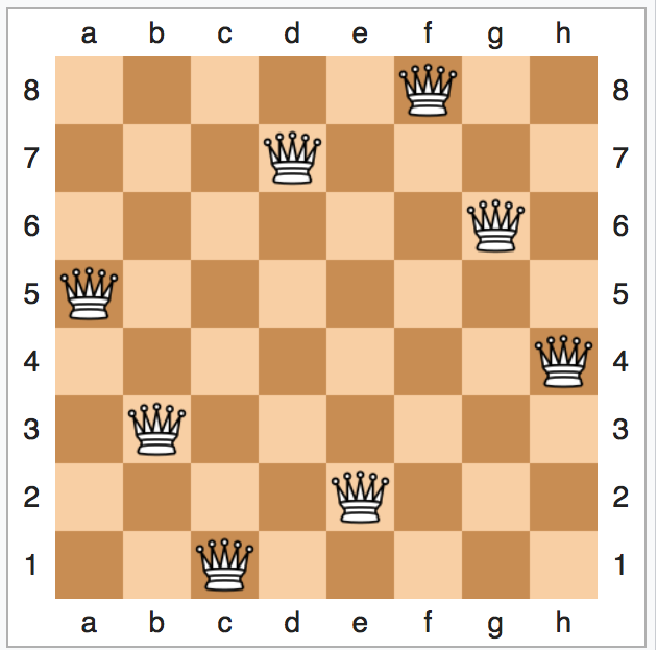
\epsfig{file=Figures/queens.pdf},
\caption{A solution of the eight queens puzzle.}
\label{fig:queens.pdf}
\end{figure}



 \pagebreak

 \exercise
 The founder of \href{https://en.wikipedia.org/wiki/Taoism}{Taoism}, the Chinese philosopher
 \href{https://en.wikipedia.org/wiki/Laozi}{Laozi} once said:
 \\[0.2cm]
 \hspace*{1.3cm}
 \textsl{``A journey of a thousand miles begins but with a single step''}.
 \\[0.2cm]
 This proverb is the foundation of \blue{taoistic search}.  The idea is, instead of trying to reach
 the goal directly, we rather define some intermediate states which are easier to reach than the goal state and
 that are nearer to the goal than the start state.  To make this idea more precise, consider the following instance of the
 15-puzzle, where the states $\texttt{Start}$ and $\texttt{Goal}$ are given as follows:
 \begin{verbatim}
        Start :=  +---+---+---+---+    Goal :=  +---+---+---+---+
                  |   |15 |14 | 8 |             |   | 1 | 2 | 3 |
                  +---+---+---+---+             +---+---+---+---+
                  |12 |10 |11 |13 |             | 4 | 5 | 6 | 7 |
                  +---+---+---+---+             +---+---+---+---+
                  | 9 | 6 | 2 | 5 |             | 8 | 9 |10 |11 |
                  +---+---+---+---+             +---+---+---+---+
                  | 1 | 3 | 4 | 7 |             |12 |13 |14 |15 |
                  +---+---+---+---+             +---+---+---+---+
 \end{verbatim}
 In order to solve the puzzle, we could try to first move the tiles numbered with $14$ and $15$ into the lower right
 corner.  The resulting state would have the following form:
 \begin{verbatim}
                  +---+---+---+---+
                  | * | * | * | * |
                  +---+---+---+---+
                  | * | * | * | * |
                  +---+---+---+---+
                  | * | * | * | * |
                  +---+---+---+---+
                  | * | * |14 |15 |
                  +---+---+---+---+
 \end{verbatim}
 Here, the character ``\texttt{*}'' is used as a wildcard character, i.e.~we do not care about the actual
 character in the state, for we only want to ensure that the first two tiles are positioned correctly.  Once we have reached a
 state specified by the pattern given above, we could then proceed to reach a state that is described by the
 following pattern:


 \begin{verbatim}
                  +---+---+---+---+
                  | * | * | * | * |
                  +---+---+---+---+
                  | * | * | * | * |
                  +---+---+---+---+
                  | * | * | * | * |
                  +---+---+---+---+
                  |12 |13 |14 |15 |
                  +---+---+---+---+
 \end{verbatim}
 We have now solved the bottom line of the puzzle.  In a similar way, we can try to solve the line above the
 bottom line.  After that, the next step would then be to reach a goal of the form
 \begin{verbatim}
                  +---+---+---+---+
                  | * | * | 2 | 3 |
                  +---+---+---+---+
                  | * | * | 6 | 7 |
                  +---+---+---+---+
                  | 8 | 9 |10 |11 |
                  +---+---+---+---+
                  |12 |13 |14 |15 |
                  +---+---+---+---+
\end{verbatim}
The final step would then solve the puzzle.  I have prepared a framework for taoistic search.  The file
\\[0.2cm]
\hspace*{1.5cm}
\href{https://github.com/karlstroetmann/Artificial-Intelligence/blob/master/Python/Taoistic-Search-Frame.ipynb}{\texttt{Python/Taoistic-Search-Frame.ipynb}}
\\[0.2cm]
from my github repository at
\href{https://github.com/karlstroetmann/Artificial-Intelligence/}{\texttt{https://github.com/karlstroetmann/Artificial-Intelligence}} \linebreak
contains a framework to solve the sliding puzzle using taoistic search where some functions are left unimplemented.  
 Your task is to implement the missing functions in this file and thereby solve the puzzle.
 \eox

%%% Local Variables:
%%% mode: latex
%%% TeX-master: "artificial-intelligence"
%%% eval: (setenv "LANG" "en_US.UTF-8")
%%% End:
